% REMEMBER: You must not plagiarise anything in your report. Be extremely careful.
\documentclass{l4proj}

    
%==============================================================================
% Put any additional packages here
% You can add any packages you want, as long as it does not alter
% the overall format (e.g. don't change the margins or the reference style).
%
\usepackage{pdfpages} % if you want to include a PDF for an ethics checklist, for example
%
%

\sisetup{
	round-mode = places,
	round-precision = 2
}

\begin{document}

%==============================================================================
%% METADATA
\title{Look At The Sky: An Audio Augmented Reality Weather App} % change this to your title
\author{Laura Henry}
\date{\today}

\maketitle

%==============================================================================
%% ABSTRACT
\begin{abstract}
   Audio augmented reality can utilise spatial audio to provide the user with helpful information about their environment without obscuring their vision. In the past, applications of the technology required highly specialised equipment and was often limited by location. More recent examples have taken advantage of smartphones and commercially available personal audio equipment, yet their uses remain specialised and typically unsuitable for everyday use in the way a standard smartphone app may be. The subject of this report, called Look At The Sky, is a prototype weather app that utilises spatial audio and head-tracking to help the user hear the current and forecast weather in 3D. User evaluation suggested that this solution could be useful. In certain use cases however the system suffered issues with gesture comfort and difficulty in translating certain weather conditions to pure sound limits its potential usefulness.
\end{abstract}

%==============================================================================
%% ACKNOWLEDGEMENTS
\chapter*{Acknowledgements}


Thank you to Conor, who never stopped supporting me throughout all of my time at university.
Thank you to my supervisor, Stephen Brewster, for your support in this process and for helping me arrange an emergency laptop loan at short notice.
%==============================================================================

% EDUCATION REUSE CONSENT FORM
% If you consent to your project being shown to future students for educational purposes
% then insert your name and the date below to  sign the education use form that appears in the front of the document. 
% You must explicitly give consent if you wish to do so.
% If you sign, your project may be included in the Hall of Fame if it scores particularly highly.
%
% Please note that you are under no obligation to sign 
% this declaration, but doing so would help future students.
%
\def\consentname {Laura McCallum Henry} % your full name
\def\consentdate {\today} % the date you agree
%
\educationalconsent


%==============================================================================
\tableofcontents

%==============================================================================
%% Notes on formatting
%==============================================================================
% The first page, abstract and table of contents are numbered using Roman numerals and are not
% included in the page count. 
%
% From now on pages are numbered
% using Arabic numerals. Therefore, immediately after the first call to \chapter we need the call
% \pagenumbering{arabic} and this should be called once only in the document. 
%
%
% The first Chapter should then be on page 1. 

% PAGE LIMITS
% You are allowed 40 pages for a 40 credit project and 30 pages for a 
% 20 credit report. 
% This includes everything numbered in Arabic numerals (excluding front matter) up
% to but *excluding the appendices and bibliography*.
%
% FORMATTING
% You must not alter text size (it is currently 10pt) or alter margins or spacing.
% Do not alter the bibliography style. 
%
%==================================================================================================================================
%
% IMPORTANT
% The chapter headings and structure here are **suggestions**. You don't have to follow this model if
% it doesn't fit your project. Every project should have an introduction and conclusion,
% however.  If in doubt, your supervisor can give you specific guidance; their view takes precedence over
% the structure suggested here.
%
%==================================================================================================================================
\chapter{Introduction}

% reset page numbering. Don't remove this!
\pagenumbering{arabic} 

% You can use \todo{} to mark text that needs to be fixed. Anything inside will appear as highlighted 
% text in the final copy, and you will also get warnings when you compile (so you don't
% forget to take them out!)

\section{Motivation \& Goals}
Augmented Reality (AR) is a traditionally visual technology that layers additional computer generated information over a user's perception. It typically demands the user's full attention to read and take in the information being presented to them either on an expensive head-mounted display or mobile phone screen.

Audio augmented reality (Audio AR) instead uses sound to communicate this information to the user, thereby freeing up their field of view.  Previous applications of the software are often designed for very specific use cases and can require specialised hardware to work.

This project aimed - through the design, evaluation and analysis of an audio augmented reality application - to investigate the viability of the technology in a general, everyday use context.

The report details a smartphone application named 'Look At The Sky' that runs on the Unity engine and utilises the Bose AR platform for spatial audio and head tracking. Look At The Sky attempts to translate a common use for a smartphone (checking the weather) into an audio augmented reality experience that could reasonably by used on a day-to-day basis.

\section{Report Overview}
\begin{itemize}
    \item \textbf{Background: }An overview of existing work in the field of Audio Augmented Reality and related spaces.
    \item \textbf{Analysis \& Requirements: }The process of deriving the necessary requirements for this project from the initial brief.
    \item \textbf{Design: }A high level discussion of the design and design process followed throughout the project.
    \item \textbf{Implementation: }A description of specific implementation details
    \item \textbf{Evaluation: }A discussion of the experiments conducted to evaluate aspects of the product, and their results.
\end{itemize}


%==================================================================================================================================
\chapter{Background}
%What did other people do, and how is it relevant to what you want to do?
In this chapter I discuss concepts relating to the topic of this paper as well as previous works in the field of Audio Augmented Reality.

\section{Audio Interfaces \& Design}

\subsection{Earcons \& Auditory Icons}
In audio interfaces, sounds can largely be split into two major groups - Earcons and Auditory Icons.

\subsubsection{Auditory Icons:} \label{subsec:auditory_icons}
Auditory Icons are designed to emulate sounds that can be heard in the real world. They represent their function in the same way a visual icon on an interface would. \cite{gaver_sonicfinder_1989} both developed and demonstrated the concept in The SonicFinder, a prototype system for the Apple Macintosh computer that provided auditory feedback when interacting with files in the Finder. The sound effect would give information about the type and size of the file in a way that the user would naturally be able to form associations between the nature of the sound and the interaction.
\begin{quote}
    "So text files might always sound wooden, whether they are selected, moved, copied, or deleted. In this way, a rich system of auditory icons may be created that relies on relatively few underlying metaphors."
\end{quote} \citep{gaver_sonicfinder_1989}

Auditory icons are particularly powerful when the information or interaction being represented already has a strong association to a sound in the real world. 

\subsubsection{Earcons:} \label{subsec:earcons}
Earcons are typically more abstract than auditory icons. They are synthetic, often melodic tones used to represent an interaction or operation on an interface. \cite{blattner_earcons_1989} likened them to the auditory twin of more abstract visual icons built with the basic building blocks of simple geometric shapes and markings. 

These basic component parts can be swapped and rearranged to create combinations of earcons that communicate related functions. For example, an earcon representing a particular file type could be combined with another earcon that generally indicates deletion to represent deletion of a file of that type. This technique can help the user to build powerful associations between related operations on the interface.

\cite{brewster_evaluation_1993} expanded upon the previous work of Blattner et al. by evaluating the effectiveness of earcons in interface design. Their work concluded that earcons were effective elements to include in an interface and that users were typically good at remembering their meaning in the short term. 

Earcons have the added advantage over auditory icons of not being tied to the use of sounds present in the user's everyday reality outside of the interface, which can allow more complex or abstract operations to be represented in audio.

\subsection{Spatial Audio}
Spatial Audio (or 3D audio) is sound that has direction in a 3D space. This is a useful component in an auditory interface as it allows the sound to intuitively communicate direction. By mapping a specific area to a function of the interface and using sound from that direction to communicate the function, much in the way that a function could be mapped to a labelled button on a graphical interface, interfaces can be built that require no visual components at all.

\cite{brewster_multimodal_2003} investigated the use of spatial audio in mobile auditory interfaces by comparing different methods of presenting audio to the user. Their experiment used a pair of headphones with an externally mounted motion sensing unit to track the wearer's head movements. Participants were presented with three different versions of the same interface - a simple dashboard that used a set of auditory icons to represent different items - in three different configurations. The participant would use head gestures in the direction of these icons to select different targets on the interface.

Egocentric design, where the sounds stayed fixed to the user's head, was found to have the least impact on mobility during use but severely limited the amount of individual targets that could be included in the interface.

Exocentric design, where the sounds stayed in their own position independent of the user's orientation allowed for larger targets and could comfortably fit more than 4 different audio targets.

\section{Early Examples}

Early examples in this space often required a lot of cumbersome external hardware specific to the system in use which severely limited its use outwith these specialised environments.

\subsection{Audio Guides}
\cite{bederson_audio_1995} investigated the viability of using an audio augmented reality system as a replacement for traditional audio guides often rented to visitors at museums and other exhibitions, which stored its audio recordings on a tape that linearly guided guests through exhibits.

The system described by Bederson allowed users to hear information about exhibits in their chosen order, which was not possible using a tape player. 

Visitors to an exhibit would wear on their person a microprocessor and infrared receiver attached to an audio device. Infrared transmitters positioned above exhibits would communicate with the microprocessors via the receivers to select an audio track for the wearer to hear. Parties visiting together could ensure that they heard the same information by approaching the exhibit at the same time.

\begin{figure}[htb!]
    \centering
    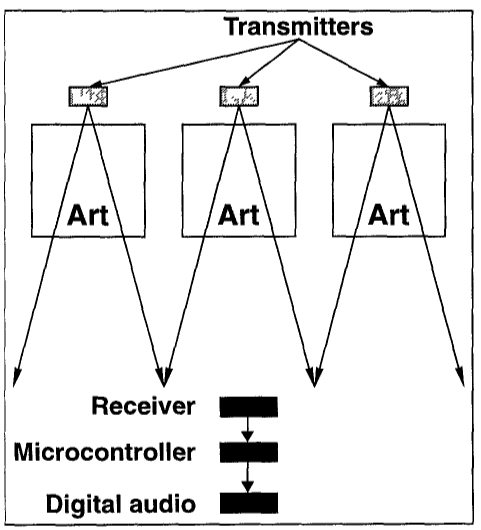
\includegraphics[width=0.5\linewidth]{images/bederson_diagram.png}
    \caption{Diagram illustrating the components of Bederson's prototype. \citep{bederson_audio_1995}}
    \label{fig:my_label}
\end{figure}

Unfortunately, no formal user testing or evaluation was conducted on this prototype, so its effectiveness and usability was not measured in this study.

\subsection{Audio Aura}
Audio Aura, a prototype Audio Augmented Reality system designed for use in the workplace, is detailed by \citet{mynatt_designing_1998} in \textit{Designing Audio Aura}. 

The system was designed as a way for employees at Palo Alto Research Center (PARC) to receive audio cues representing certain notifications like unread emails or indicating if a given colleague has recently been in their office. 

Audio Aura deliberately avoided sharp, alarm-like notification sounds and instead tried to keep its audio design gentle and non-intrusive as users went about their daily workflow. The system offered three main audio modes, each with different types of sound cues, as well as a combination of all three in another mode. 
\begin{itemize}
    \item \textbf{Sound Effects} mode used naturalistic sound design, mapping notifications to different elements of a beach soundscape such as the calling of seagulls to indicate new messages. Though these are examples of auditory icons, the user would still need time to build up their mental model of what each part of the soundscape represents since beach sounds would not be intuitively associated with workplace notifications. In their user test, the Audio Aura team did find that participants found the meaning of the sounds "difficult to remember" \citep{mynatt_designing_1998}.
    \item \textbf{Music} mode utilised melodic earcons in its audio design. These were found to require some time and energy on the user's part to learn what each distinct earcon indicated in this mode. 
    \item \textbf{Voice} mode gave verbal notifications to the user. This mode commanded significantly more of the user's attention when in use than the other audio modes, but was more naturally intuitive through its use of simple language. The user did not have to figure out what these sounds were trying to convey.
\end{itemize}

The system relied on extensive existing infrastructure at PARC. Employees wore location tracking badges that communicated with a central server via infrared signals and an extensive array of sensors located throughout the building. Audio Aura built on these existing systems to run queries against the data provided by the badges. This reliance on the client/server design and the large amount of specialised hardware required to make the system work limited Audio Aura's use outside of specifically configured locations.

\section{Modern Examples}
Modern examples of audio augmented reality tend to rely less on proprietary infrastructure and more on commercially available technologies, particularly smartphones.

\subsection{PULSE \& Social Applications}

\cite{mcgookin_pulse_2011} detailed a prototype iOS application named PULSE, which aimed to utilise social media data to help its users gauge the "vibe" of a certain location through a spatialised auditory display. 
PULSE aggregated related Twitter activity from the same small area (around 100m radius) and played audio cues to the user to indicate the online activity in that area.

McGookin and Brewster investigated two distinct ways of presenting this information: explicit presentation and implicit presentation. Implicit presentation informed the user about the volume, density and diversity of the activity by varying the existing sound cues, for example by varying the speed at which they were played to the user. Explicit presentation, on the other hand, represented these different elements using different sound effects of a water soundscape and varying them as needed, similarly to the design of audio aura. Explicit presentation was found to fix many issues found in the implicit design by allowing more detailed information to be presented to the user and at a higher speed than was allowed when using implicit presentation.

An issue faced during the development of PULSE was the choice of soundscape since it needed to fit naturally into whichever environment the app was used in. Water was chosen since it can be found in both urban and rural areas.
\subsection{Multimodality \& Accessibility in Audio AR}
Audio Augmented reality has also proved a valuable tool in designing interfaces for visually impaired users. 

\cite{puiatti_whats_2012} proposed a mobile application named \emph{In Situ Audio Services} (ISAS), which was specifically designed to help blind users discover points of interest in their environment, such as restaurants and shops using spatialised audio effects.

ISAS was intended to be widely available to its target audience and so only requires a standard smartphone to run the application and a pair of headphones. This directly opposed many available systems for visually impaired users at the time, many of which required expensive, specialised hardware that wasn't widely distributed.

Spatialised audio is crucial to the functionality of this system as it provides the user with information on the direction and proximity on potential points of interest in their environment while requiring a lower cognitive load than standard spoken directions like those found in most standard navigation systems \citep{klatzky_cognitive_2006}. Similarly to Audio Aura, ISAS' focus laid on providing information to the user on the edge of their aural perception. Both systems encouraged users to naturally take notice of their audio environment, rather than immediately demanding their full focus with overly detailed descriptions of what each sound represented.

\subsection{Bose AR}
Audio hardware manufacturer Bose first announced its augmented reality platform at the South By Southwest conference in March of 2018 \citep{corporation_bose_2018} alongside a prototype of the first generation Bose Frames. Bose AR focused on freeing up the user's visual attention and moving information that would typically be displayed on a screen or head mounted display in traditional AR situations to a purely auditory interface.

One of the main benefits of the Bose AR platform was that it required a pair of compatible consumer headphones and a mobile phone running a supported application to work. Compared to earlier examples of audio augmented reality which often required proprietary hardware to use, Bose's approach greatly widens the reach of the technology to the general user.

A large portion of Bose's efforts regarding their new AR platform concentrated on the augmented reality gaming space, which had previously seen little innovation in terms of audio-only content. Multiple games were created as a result of this effort, typically utilising the gesture capabilities of the supported hardware to create eyes-free experiences \citep{takahashi_bose_2019}. 

However, this focus on games meant that little was being done to accommodate the general user. In a final statement in 2020 before the project's cancellation, a spokesperson for the company said:
\begin{quote}
    "We learned a lot - mostly, that our work in AR delivered compelling customer experiences based on specific interests and specific use cases, not for broad, daily use."
\end{quote} \citep{roettgers_another_2020}

Bose officially stopped supporting their AR ecosystem in June of 2020, only around 2 years after its announcement \citep{roettgers_another_2020}, and the Bose Developer Platform closed down permanently. Though the development kit can still be used and is still compatible with previously AR-enabled Bose devices, the full documentation, manuals and developer forums are no longer available.

%==================================================================================================================================
\chapter{Analysis \& Requirements}
%What is the problem that you want to solve, and how did you arrive at it?
This chapter describes the process and outcomes of deriving implementation requirements for this project.

\section{Tasks}
The overall aim of this project was to explore and demonstrate a new possible application of audio augmented reality in an everyday usage context.

This meant creating a product that users could conceivably want to use in their day-to-day lives, while utilising the technology in a creative and useful way. 

\section{Constraints}
When narrowing down the possible space of projects, several design constraints needed to be taken into consideration in order to successfully and creatively meet the goals of the project.

\subsection{Mobile Application}
A mobile application made the most sense for this project since the final product was to be usable in a variety of environments. Keeping the app on a mobile platform would allow it to make use of the Bose AR SDK - which requires Bluetooth Low Energy (BLE) on either iOS or Android to connect to the supported headsets and use their sensor data. 

Given the equipment available during development, it was decided that the final product would be an application for Android devices.

\subsection{Make Use Of The Hardware}The product should take advantage of the capabilities of the audio augmented reality hardware as much as possible and in an interesting way.
This includes: \begin{itemize}
    \item Utilising the sensor unit to allow gesture-based interaction.
    \item Making the audio integral to the functionality of the app, not just supplementary.
    \item Taking advantage of spatial audio capabilities.
\end{itemize}
When brainstorming the concept, it was important that the audio augmented reality hardware was considered at every step. Gesture interaction was important to include as it reduced the reliance the user had on looking at their mobile device's screen for information or needing to pull their focus away from the audio experience to use button inputs to access the basic features of the app.

The decision to use gesture inputs for an app designed for general, everyday use meant that considerations needed to be made about the social acceptability of the system - therefore gestures could not be so complex that they would make the user feel nervous or be difficult to perform while moving.

\subsection{Augment Reality, Don't Change It}

The audio should form a natural part of the user's auditory perception and shouldn't demand too much focus to communicate the intended information.

The sounds themselves should not seem too out of place so the sound design should be kept as naturalistic as possible. They should emulate sounds that the user may expect to hear in their everyday environment. This meant keeping the use of abstract or purely verbal sounds as limited as possible and considering what environment the app may be used in when designing the soundscape.

\section{Solutions}

The proposed solution, named 'Look At The Sky', is a mobile weather app that plays an immersive 3D sound effect representing the current weather when the user looks up.
Using the tasks and constraints detailed above, I was able to derive a set of functional and non-functional requirements prioritised according to the MoSCoW methodology \citep{kravchenko_ranking_2022}.

\subsection{Functional Requirements}

These functional requirements define \emph{what} the final product will be able to do.
\begin{itemize}
    \item \textbf{Must} connect to AR enabled headsets over Bluetooth and utilise their audio and motion sensing capabilities.
    \item \textbf{Must} play spatial audio representing the current weather when the user looks up.
    \item \textbf{Must} play audio representing upcoming weather in positions relating to how far in the future that weather will be.
    \item \textbf{Should} represent a wide range of weather conditions
    \item \textbf{Should} provide aural or visual feedback to the user to help them ensure that the hardware is functioning correctly.
    \item \textbf{Could} allow users to customise some of the parameters of the gesture detector to their preference and comfort.
    \item \textbf{Could} allow users to choose how many forecast weather effects are included in the forecast mode.
    \item \textbf{Could} play a subtle audio notification to the user if it is going to rain.
    \item \textbf{Would be nice to} Provide supplementary information about the weather i.e. temperature, humidity etc.
    \item \textbf{Would be nice to} allow the user to customise aspects of the audio i.e. volume or fade-in.
    
\end{itemize}

\subsection{Non-Functional Requirements}
These non-functional requirements define \emph{how} the final product will present and perform its functions.
\begin{itemize}
    \item \textbf{Must} utilise gesture control that is easy for the user to perform.
    \item \textbf{Must} present a user interface that is easy and intuitive for the user to navigate.
    \item \textbf{Should} position sound objects in such a way that the user can distinguish their direction.
    \item \textbf{Should} intuitively communicate the intended weather condition using naturalistic audio.
    \item \textbf{Should} not demand too much of the user's attention so that they are still aware of their surroundings.
    
\end{itemize}

%==================================================================================================================================
\chapter{Design}
%How is this problem to be approached, without reference to specific implementation details? 

In this chapter I describe the high-level design of the application, the approach taken to design throughout the project and how the design evolved.

\section{Overview}

Look At The Sky is a mobile app that uses immersive 3D sound to communicate the current and forecast weather.

There are two main interactions that the user can perform:
\begin{itemize}
    \item A \textbf{look up} gesture to hear a detailed 3D sound effect representing the current weather that lasts for as long as the user looks up.
    \item An \textbf{input} gesture to toggle a forecast view, where the current and forecast weather effects are positioned in a 360$^\circ$ ring around the user's head.
\end{itemize}

\subsection{Current Weather}

The application uses primarily head gesture based interaction to free up the user's visual space and encourage them to focus on the sounds rather than their smartphone's screen.

The user can look up to hear a 3D sound effect that represents the current weather. The effect continues to play for as long as the user is looking up. The look up gesture fits well as an interaction method for this app as it is a simple gesture for most users to perform that intuitively relates to checking the weather.

\begin{figure}[htb!]
    \centering
    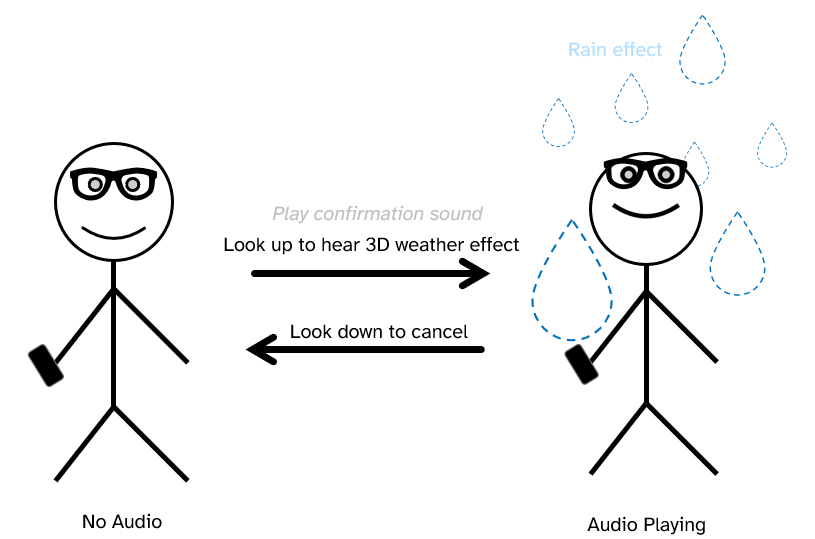
\includegraphics[width=0.8\linewidth]{images/main_interaction_diagram.png}
    \caption{Illustration depicting the main gesture control flow found in the app.}
    \label{fig:main_interaction_diagraml}
\end{figure}

\subsection{Forecast Mode}

The forecast view is a separate mode with slightly different functionality to the standard mode. It is a way to 'view' both the current and upcoming weather by positioning the weather effects in a circle around the user's head in a clock-like fashion. The effect positioned directly in front of the user is the current weather and every subsequent position represents an hour ahead of the last.

It can be toggled on and off by performing an 'input' gesture that varies slightly depending on the headset.

\begin{figure}[htb!]
    \centering
    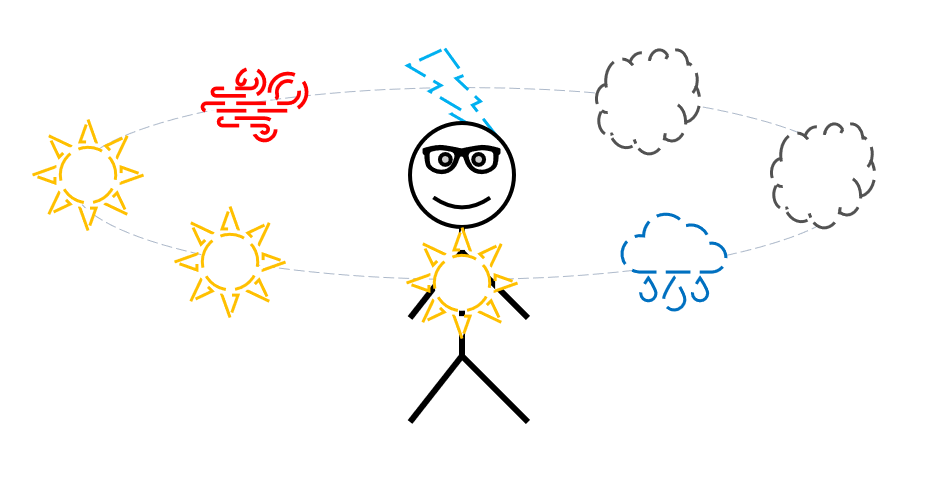
\includegraphics[width=0.9\linewidth]{images/forecast_illustration.png}
    \caption{An illustration depicting the app's 'forecast mode'}
    \label{fig:forecast_illustration}
\end{figure}

\section{Design Process \& Prototyping}

The design of the app was very fluid and continued to evolve throughout the entire development and design process.
\subsection{Early Design}

Much of the early design work utilised paper prototyping as a way to generate ideas quickly. Figures \ref{fig:early_paper_prototype} and \ref{fig:paper_prototype_1} show some of these design concepts.

\begin{figure}[htb!]
    \centering
    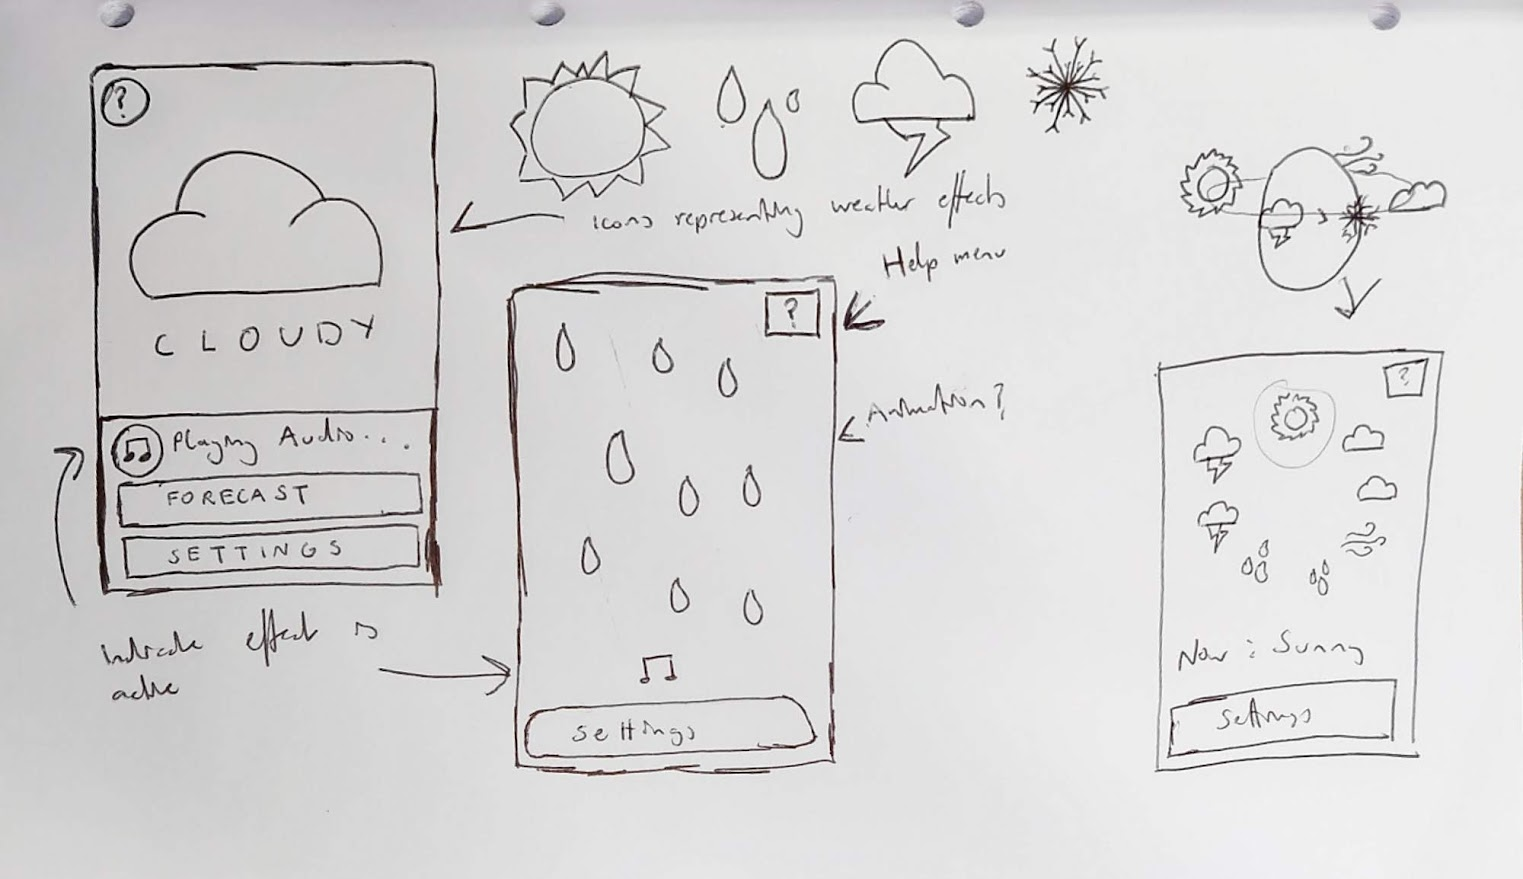
\includegraphics[width=0.9\linewidth]{images/early_paper.jpg}
    \caption{An early paper prototype showing a mostly 2-dimensional design. Weather conditions are represented by 2-dimensional icons or animations. These designs were inspired by existing widely available weather apps.}
    \label{fig:early_paper_prototype}
\end{figure}

The design shown in Figure \ref{fig:early_paper_prototype} is more akin to commonly available weather apps and uses mainly 2D icons and animations to communicate the weather to the user.

The Forecast view is reminiscent of a clock, with the current weather at the 12 o'clock position and then positioning subsequent weather effects in a clockwise direction.

\begin{figure}[htb!]
    \centering
    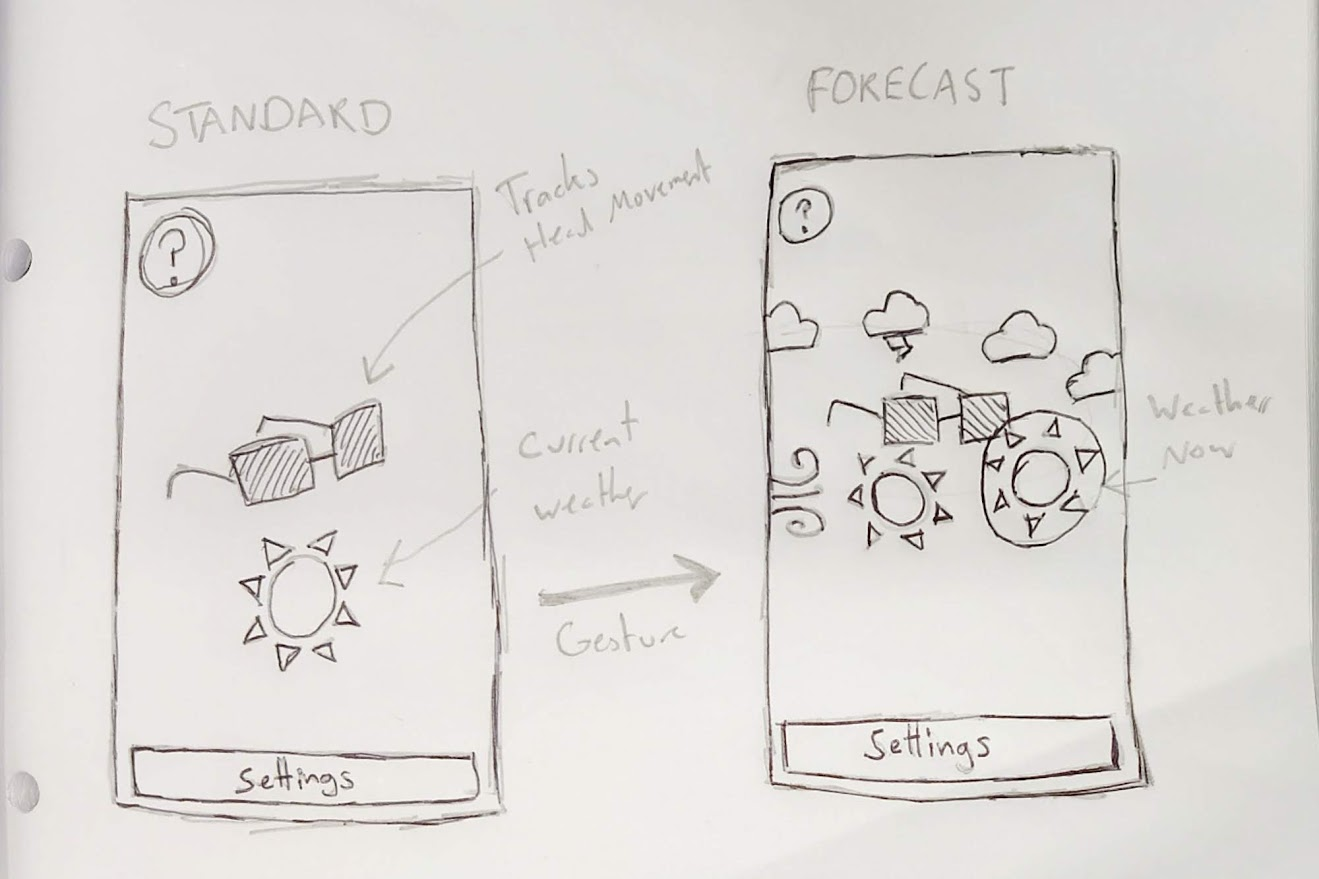
\includegraphics[width=0.9\linewidth]{images/paper_proto_1.jpg}
    \caption{A later paper prototype. This adds in a model of the headset that mirrors the movement of the user's head. In forecast mode, the position of each sound in the space around the device is shown with an icon representing that weather condition.}
    \label{fig:paper_prototype_1}
\end{figure}

Figure \ref{fig:paper_prototype_1}'s design is a lot closer to the final product, though elements were added and altered throughout the process. 
This design creates a 3D space for many of its UI elements to exist in, most importantly allowing a model of the connected headset to reflect the gyroscope data from the device. This provides feedback to the user that the device is connected and properly tracking their head movements.

The forecast mode in this design also takes advantage of the 3D environment by showing the circle of weather icons in a ring around the headset model so the user can easily tell which they are looking at - though the space around the headset runs the risk of becoming overcrowded with icons.


\subsection{Iteration \& Improvement}

The design of the app evolved throughout the design and implementation stages as I became more familiar with the toolset.

During the early stages of implementation I made use of a basic menu to switch between different weather effects before implementing the system to read in weather conditions from an external data set. As the project progressed this became a "Demo" mode (shown in Figure \ref{fig:screenshots}) as opposed to a debug mode used purely in development as it presented a useful opportunity to allow users to try all of the available effects during evaluations. 

The final design combines elements from both sets of paper prototypes shown above, most notably in the design of the forecast view which uses the clock-like design from the earlier prototype to give each visual effect enough space while also utilising the 3D model of the headset to help the user track which effect they are facing and how far in the future that weather condition is. 2D icons are removed entirely in favour of dynamic effects that make use of the 3D space.

\begin{figure}[htb!] 
    \centering
    \begin{subfigure}[b]{0.35\textwidth}
        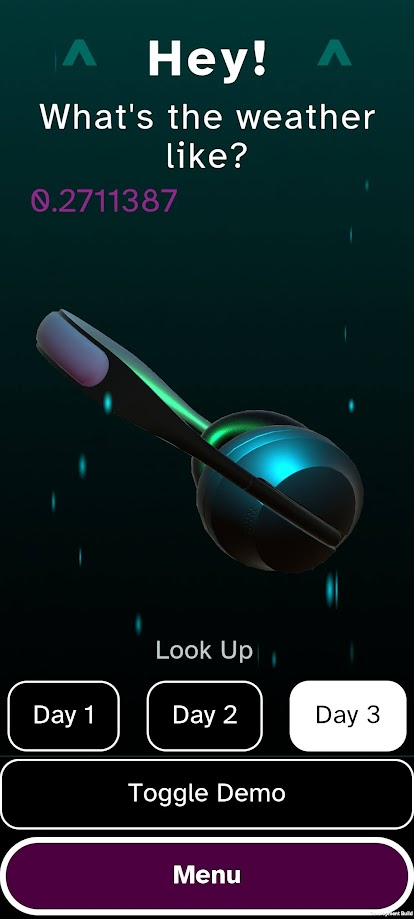
\includegraphics[width=\textwidth]{images/time_screenshot.jpg}
        \caption{An example of the app while playing a rain weather effect from one of the example day data sets.}
        \label{fig:syn1}
    \end{subfigure}
    \quad
    \begin{subfigure}[b]{0.35\textwidth}
        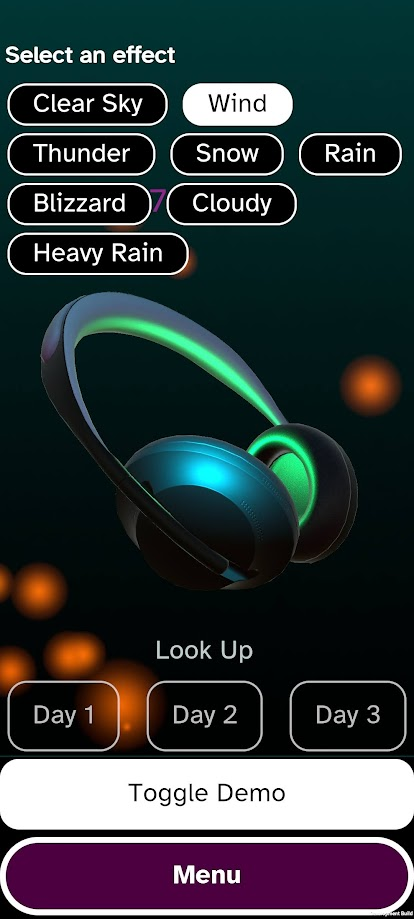
\includegraphics[width=\textwidth]{images/demo_screenshot.jpg}
        \caption{An example of the app playing a wind sound effect - selected by the user in demo mode.}
        \label{fig:syn2}
    \end{subfigure}
    \caption{Screenshots from the final working version of the app. In both, the app is connected to the NC700 Headset.
    }\label{fig:screenshots}
\end{figure}

\section{Weather Effects \& Sound Design}

The majority of sounds in the design are auditory icons (\ref{subsec:auditory_icons}) that should be able to intuitively communicate the weather condition they represent. To create an immersive experience for the user, most sounds are positioned \emph{exocentrically} - they stay at a fixed point in 3D space even as the user turns their head. 

Sound design was tackled first as it was considered the most important aspect to get done correctly as soon as possible. The effectiveness of these auditory icons were evaluated (See Section \ref{sec:audio_survey}) and the sound design was adjusted based on the results and feedback as the design and development process progressed. 

Most of the audio clips that were used in this project were sourced from online free sound effect libraries, while the remainder were included in an example project with Bose's AR tools. Attribution for these audio sources is given in Appendix \ref{adx:audiosources}.

\subsection{Clear Sky}
In an early version of the app this was the simplest of the suite of sound effects and only used one audio clip of summer birds singing, positioned directly above the user's head.

Inspiration was drawn from existing weather apps (Figure \ref{fig:accu_daynight}) to have the clear sky effect implement a day and night cycle. This involves playing sounds associated with a clear, sunny day when the effect is triggered between sunrise and sunset and sounds associated with a still night play between sunset and sunrise.

Both variations of the sound mirror each other through their use of bird calls. The daytime variant still consists of a variety of summer birds, but more have been layered to emphasise the bird song over the light breeze present in the initial clip. The nighttime variant uses a variety of owl calls since owls are often associated with the night due to their nocturnal nature.

\begin{figure}[htb!] 
    \centering
    \begin{subfigure}[b]{0.4\textwidth}
        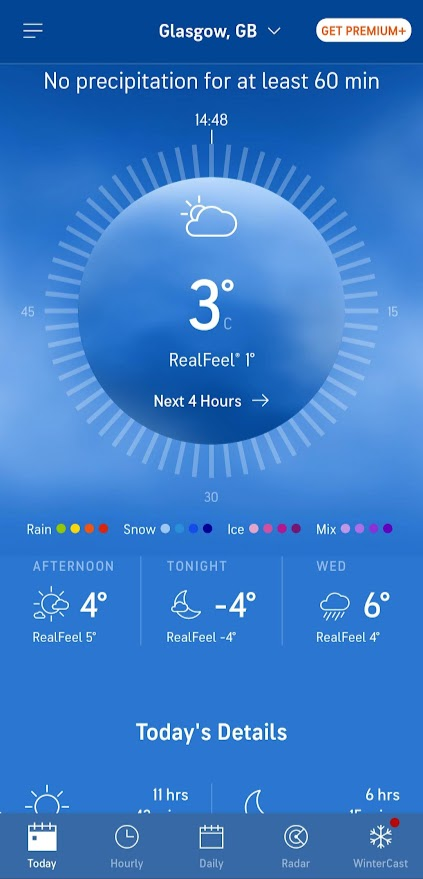
\includegraphics[width=\textwidth]{images/Accu_day.jpg}
        \caption{An example of the AccuWeather interface during the day.}
        \label{fig:syn1}
    \end{subfigure}
    \quad
    \begin{subfigure}[b]{0.4\textwidth}
        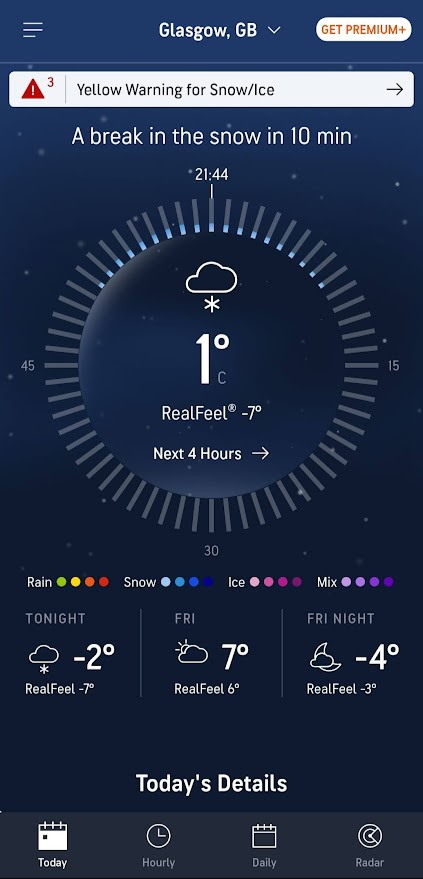
\includegraphics[width=\textwidth]{images/Accu_night.jpg}
        \caption{An example of the AccuWeather interface at night.}
        \label{fig:syn2}
    \end{subfigure}
    \caption{An example of the day/night cycle in a popular existing weather app: AccuWeather for Android. \textbf{Images: }\cite{accuweather}
    }\label{fig:accu_daynight}
\end{figure}

The day/night cycle in Look At The Sky affects both the aural and visual design of this effect.

\subsection{Rain}
I decided to split rain into two separate effects - a lighter rain and a heavier rain. The rain sound was broken into individual raindrop effects as well as additional ambient noise to add to the immersion of the effect.

By breaking the sound down into individual units, I gained finer control over the speed, volume and spatial positioning of the sound. Rapidly layering these individual clips together in different positions around the user's head allowed me to create a far more immersive soundscape than if I had only played one complete 'rain' sound clip from one position.

For the heavier version of this effect the raindrops are played faster, louder and with a wider range of possible pitches.

In an earlier iteration of the app the sound used for individual raindrops was more of a traditional 'water drop' sound. This didn't sound natural at all and many available audio clips of this kind were of poor quality. As the design progressed, the audio clip used for the sound of raindrops was updated to the sound of a kick drum. The low 'impact' sound created by the drum imitates the sound of rain hitting a roof or window.

\subsection{Snow}
The snow effects (split into a gentle snowfall and more violent blizzard effect) were designed in a similar way to the rain effects described above. 

Deciding on a sound to use to represent individual snowflakes presented a challenge when designing this effect. I elected to use a bell sound to create associations with winter.  While this did successfully communicate the intended weather condition to participants in user testing, it is still not an ideal clip to use as it is more associated with Christmas than winter in general and this connection may not exist for users who don't celebrate Christmas.

I used the sound of heavy footsteps in snow moving around the user to create the impression of snow lying on the ground.

\subsection{Wind}
The most prominent audio clip used here is the sound of wind chimes. Having this be the main clip allowed the sound of wind itself to be used in the effects for other weather conditions (namely Blizzard and Clouds), while still remaining distinct and recognisable as wind.

\subsection{Thunderstorm}

The main element of the design of the thunderstorm effect is three different thunderclap sound clips from three separate positions that orbit the user's head at varying speeds.

Each clip has a different amount of silence added to give a sense of randomness as the clips loop and move out of sync with each other, while not leaving too much time without a thunder sound playing.

There is rain present in this soundscape however as it isn't the focus of this effect the volume is greatly reduced when compared to the two main rain effects.

\subsection{Cloudy}

Cloudy was the most difficult weather condition to represent as an auditory icon but it was included in the set for coverage and to test whether it could at all be represented as sound. The cloudy effect also went through the most radical changes after the initial user evaluation of the sound choices.

The early design of the cloud effect was the most abstract of all sounds and was the only effect that made use of ambient music. 
I found that this design choice poorly communicated the intended weather condition and was actively distracting to users.

This music was removed in the final version to create a more naturalistic sound in line with the rest of the suite of sound effects. The volume of the wind clip used here was turned down as it was had a deeper, more bass-heavy sound than other wind clips used in the app that was described by some participant as "ominous" and "unnatural".

\subsection{Supplementary Sounds}

Look At The Sky makes limited use of earcons (See \ref{subsec:earcons}) in the design. These provide confirmation to the user that they have successfully triggered a gesture interaction.

\subsubsection{Look Up Activated:}
A short tone that plays immediately before the weather sound starts playing. It is quiet enough that it can blend into the more intense sounds like Heavy Rain or Blizzard.

\subsubsection{Forecast Mode Activated:}
A longer collection of high tones notifies the user that the gesture had been successfully triggered and the app has switched modes.  

\subsubsection{Forecast Mode Deactivated: }
Similar to the earcon used when forecast mode is turned on, this version uses lower tones to show that forecast mode has been disabled and the user is being returned to the standard mode of the app. 
These longer earcons are played at a louder volume and indicate a major change of function, since the standard gesture control is completely disabled in forecast mode.

These supplemental earcons are the only audio clips in the app to completely lack any kind of spatiality as they don't need to immerse the user in any way.

\section{Hardware}
The project was designed for use with Bose AR supported headsets since they provide a development kit to simplify connection and interfacing with mobile devices over Bluetooth.

The Bose AR platform supports three device families:
\begin{itemize}
    \item Bose QuietComfort 35-II Headphones (QC35-II)
    \item Bose Noise Cancelling 700 Headphones (NC700)
    \item Bose Frames - the primary device family designed for AR.
\end{itemize}

This project focused on comparing the Frames to the NC700 headset.

The NC700s are fairly standard noise cancelling headphones while the Frames (shown in Figure \ref{fig:frames}) are more unusual. They are 'smart audio sunglasses' with discrete speakers that sit on the temples and point at the user's ears. This open-backed design makes the frames easier to use in situations where the user may still want to hear other sounds around them as they do not form a seal around the wearer's ears that blocks out external sounds.

Both devices are equipped with a sensor unit consisting of a gyroscope, accelerometer and magnetometer. The NC700s also have a small touch-sensitive panel on the right ear cup that can be used for gesture control.

\begin{figure}[htb!]
    \centering
    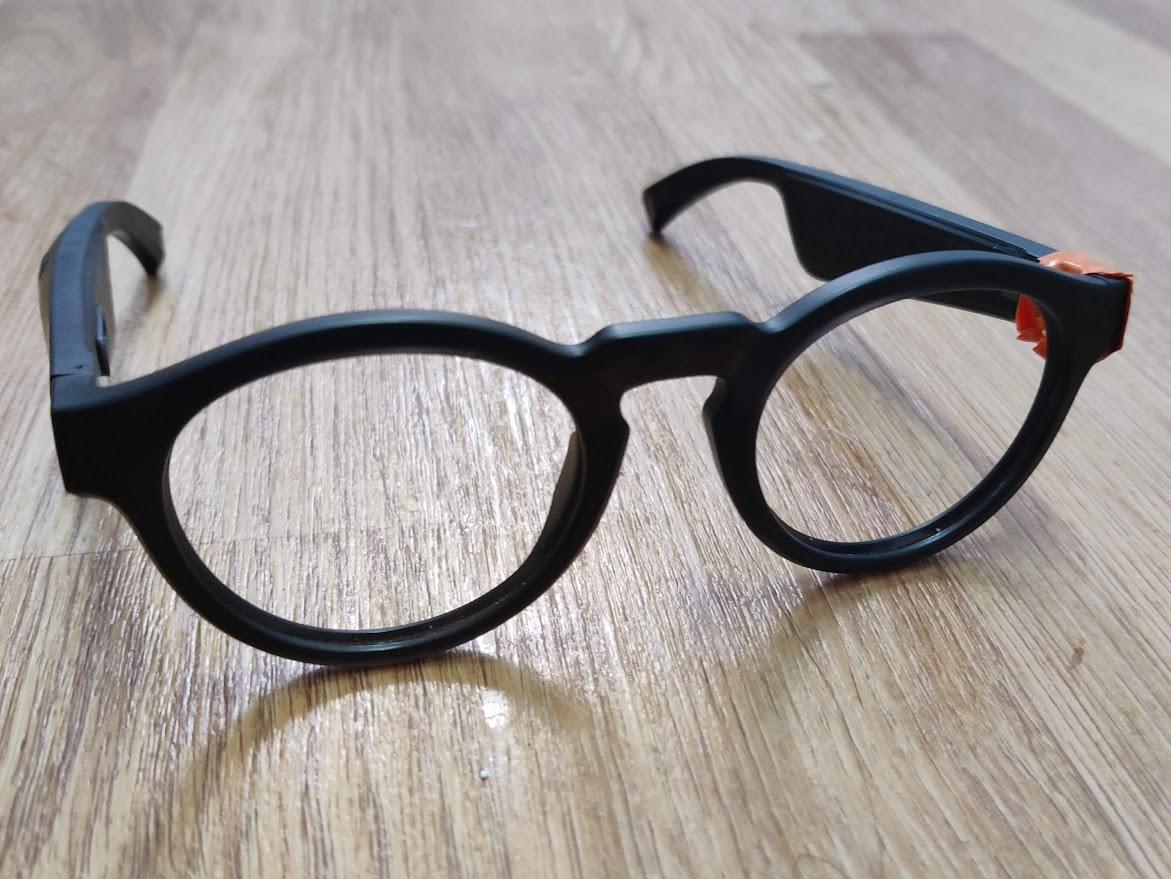
\includegraphics[width=0.6\linewidth]{images/frames.jpg}
    \caption{An image of the Bose Frames uses in this project. On typical units they would have UV-resistant lenses but these have been removed here so they do not impact the wearer's vision.}
    \label{fig:frames}
\end{figure}
%==================================================================================================================================
\chapter{Implementation}
%What did you do to implement this idea, and what technical achievements did you make?
\section{Toolset}

\subsection{Unity}
The project was developed entirely in the Unity engine, which allowed me to make use of the Bose AR SDK. Unity also already implemented a full-featured spatial audio system typically for use in video game development, but which easily laid the groundwork for spatial audio in Look At the Sky.
Any \texttt{AudioSource} object can be given a specific range that the scene's \texttt{AudioListener} must be within to allow the user to hear the clip attached to that \texttt{AudioSource}. 

\subsubsection{Bose AR SDK}
The Bose AR SDK is a development kit allowing a Unity program running on a smartphone to connect to a Bose AR enabled audio device using Bluetooth, access the stream of data from its motion sensors and play 3D audio.

For this project, Bose AR provided a way to easily create an audio augmented reality system using commonly owned devices like smartphones and noise-cancelling headphones. In addition, the SDK provided useful pre-built resources for handling the Bluetooth connection and capturing the stream of data from the on-board sensors. 

The discontinuation of support for the Bose AR SDK significantly affected decisions made during the implementation process specifically regarding certain aspects of communicating with the hardware such as recalibrating or re-centering the motion sensors. In some cases while testing the sensor data would become inverted, causing the gesture interaction to trigger when the user was looking down instead of up. I found that rotating the headset a full $360^{\circ}$ could cause this inversion of the rotation values and thus could be used to 'recalibrate' the head tracking in some cases where the gesture control was working incorrectly. This method worked far more reliably when testing using the Bose Frames than the NC700 Headphones.


\subsubsection{UI Toolkit:}
Unity's UI Toolkit is a recent addition to its suite of tools. It is an XML based UI builder similar to the Layouts system used in native Android development\footnote{Android Developer Documentation: \url{https://developer.android.com/develop/ui/views/layout/declaring-layout}} or Storyboards in iOS\footnote{iOS Documentation: \url{https://developer.apple.com/documentation/uikit/uistoryboard}}.

Look At The Sky's user interface was built using the new UI Toolkit instead of the older Canvas system as it allowed me to keep the 2D and 3D elements of the app separate and this project did not require any of the 3D capabilities of the Canvas System.


\subsection{Audacity}
Audacity is a free and open source audio editing program which provided more than enough functionality for my purposes.

A small amount of audio editing was completed in Audacity since Unity lacks the ability to cut, extend, or add finer effects to individual audio clips. Several ambient sound effects had fade-ins first applied in Audacity before they were imported into the project. Clips which required a consistent pause between loops (i.e. individual thunder clips) had silence added to the end of the file.

\subsection{Windows \& PC Issues} I faced intermittent PC issues throughout the duration of this project which often required a full re-installation of my operating system. This required diligent physical and cloud backups of my work even more so than usual as these issues would often appear without prior warning signs.

Though no data was lost, fully reinstalling the necessary tools often took several hours and led to me eventually seeking a temporary loan PC.

\section{Reading Data}
\subsection{Data Sets}
In practice, this app would fetch its data from an API such as Accuweather\footnote{Accuweather API: \texttt{https://developer.accuweather.com/apis}} or OpenWeatherMap\footnote{OpenWeatherMap API: \texttt{https://openweathermap.org/api}}. For ease of testing for this project however I opted to instead use three custom JSON files, each representing an example 24 hours of weather. This meant that the data could be easily tweaked as necessary for testing and demonstration. Having complete control of the data meant I could ensure each file was distinct from the others so users could experience multiple different effects - something which would not be guaranteed if the app simply pulled the current Glasgow weather.

\subsection{Reading from JSON}

The three JSON data sets each contain 24 entries. Each entry represents an hour of the day, given in 24 hour format, and provides an integer value specifying the weather for that hour and an integer specifying the wind angle (this is set to zero if the weather is not windy).

The \texttt{JSONReader} script handles the JSON files and converts their values to be more useful to the app. Each hour's entry is converted to an \texttt{EffectEntry} object with fields for the weather effect to play and the wind angle to set, if required. These fields are both represented by the enumerated types \texttt{WeatherEffect} and \texttt{WindAngle} respectively, and are converted directly from the integer values from the JSON file.

These \texttt{EffectEntry} objects are used as values in a dictionary structure, with the hour of that effect as the key. This structure allows for fast access to the correct effect when called upon.

\section{Gesture Detection}
Head tracking utilised the headsets' built-in Inertial Measurement Unit (IMU). I chose to use the basic gyroscope, with 6 degrees of freedom,  over the magnetometer which can provide 9 degrees of freedom but would introduce additional latency to the sensor data.

The main 'look up' interaction used a custom gesture detection script, as it is not one of the gestures built into the Bose Hardware.

\begin{figure}[hbt]
    \centering
    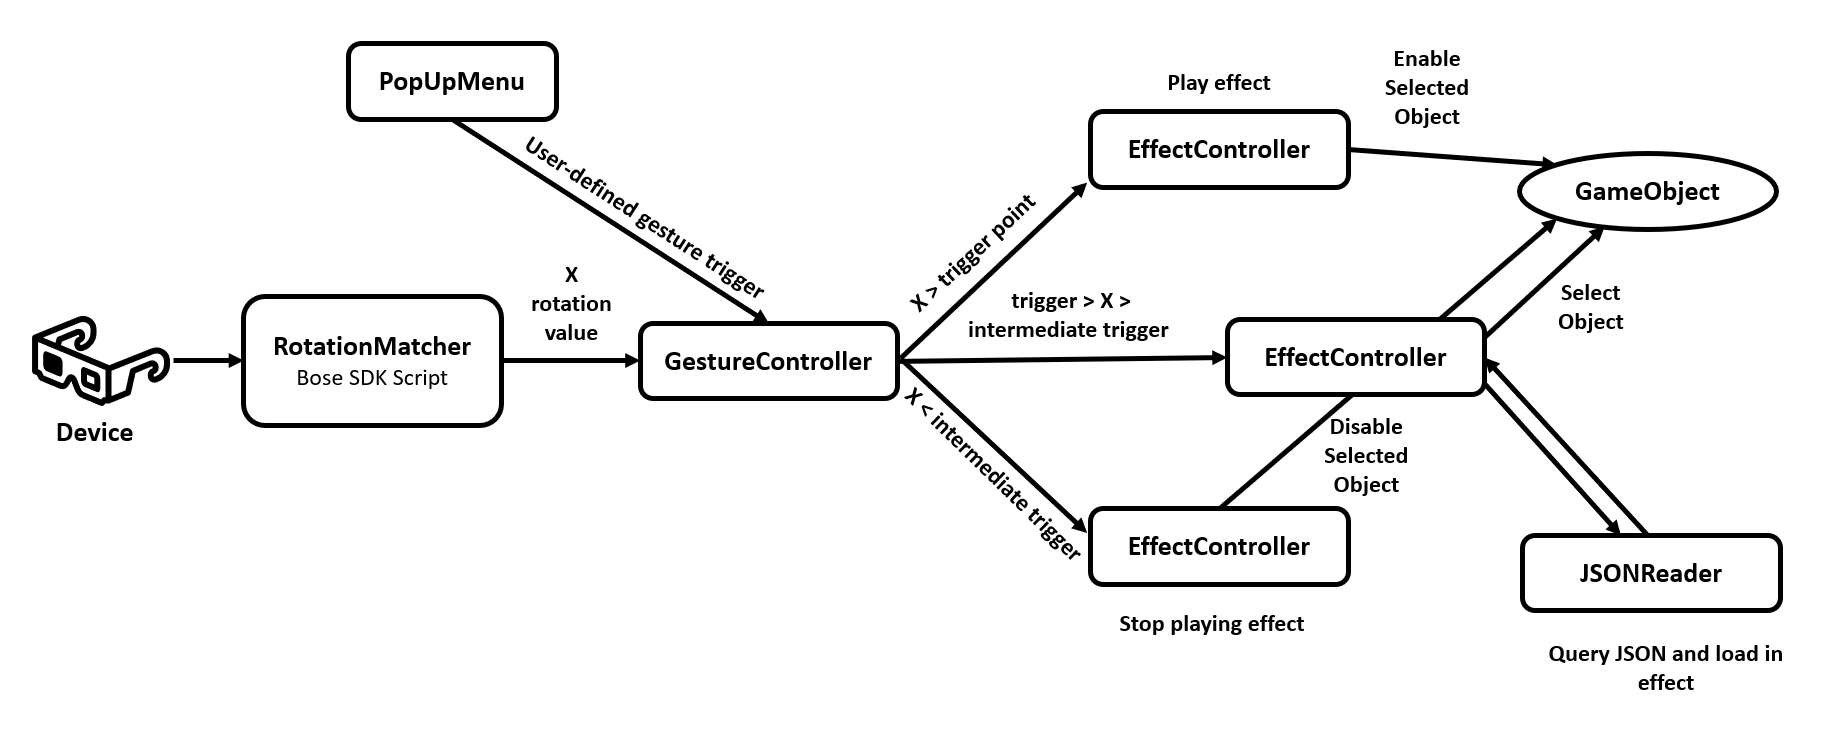
\includegraphics[width=\linewidth]{images/flow_diagram.png}
    \caption{A high-level representation of gesture control in the app. Raw data from the IMU in the headset is converted to Unity Vectors by the \texttt{RotationMatcher} script (included in the Bose SDK). The X rotation value is passed to the \texttt{GestureController}. On every frame update, the \texttt{EffectController} script is invoked to enable, disable, or reload the desired sound effect depending on the rotation of the device.}
    \label{fig:gesture_flow_diagram}
\end{figure}

Bose's \texttt{RotationMatcher} script, which allows the on-screen model of the connected headset to mirror the movements of the physical device, was also used to convert the raw values from the IMU into Unity's quaternion rotation system.

The custom script \texttt{GestureController} monitors this rotation vector from \texttt{RotationMatcher} and calls the appropriate method in the \texttt{EffectController} script.

The two main variables passed into the \texttt{GestureController} are the \textbf{Trigger Point} and the \textbf{Effect Delay}, which is used to derive the \textbf{Intermediate Trigger}. 
\begin{itemize}
    \item The \textbf{trigger point} is the rotation value at which the gesture is triggered and the appropriate weather effect object is enabled. It is initialised based on the connected headset as the rotation translates slightly differently for each and can be adjusted by the user in the settings menu.
    \item The \textbf{effect delay} is the distance the head can be brought down past the trigger point before the active weather effect is turned back off. This delay gives the user some more freedom of movement after activating the gesture and ensures the effect doesn't immediately turn back off. The delay can be customised by the user in the settings menu.
    \item The \textbf{intermediate trigger} is the \emph{effect delay subtracted from the trigger point}. The intermediate trigger has different functions depending on whether the weather effect is being enabled or disabled. When the effect is being enabled, the intermediate trigger is the point at which the correct effect is loaded from the JSON files. Otherwise this is the rotation value at which the active effect is disabled.
\end{itemize}

Since \texttt{GestureController} monitors the rotation vector on every frame update (approximately 60 checks every second), various boolean checks are incorporated to prevent unnecessary duplicate calls to \texttt{EffectController}. Listing \ref{lst:gesture_update} shows the \texttt{Update()} method, where the main logic of the \texttt{GestureController} is implemented.

%Note: In this case java syntax highlighting can be used as listing doesn't seem to like C# and nothing C# specific is used.
\begin{lstlisting}[language=java, float, caption={GestureController's Update() method which hands off to the EffectController based on the current rotation of the device.}, label=lst:gesture_update]
    // Update is called once per frame
    void Update()
    {
        if (isEnabled)
        {
            _xpoint = transform.rotation.x;

            if (_xpoint > triggerPoint)
            {
                _inZone = true;
                GestureTriggered(); //Enable Effect
            }
            else if
                (_xpoint >
                 _intermediateTrigger)
                 //The intermediate trigger sets the effect on the upswing and gives the user more neck freedom on the downswing
            {
                if (!_effectSet) //Has the effect been loaded?
                {
                    if (!debugMode) //Are we in demo mode?
                    {
                        effectController.SetEffect(); //Load effect from JSON
                        _effectSet = true;
                    }
                }
            }
            else
            {
                effectController.exitZone(); //Disable Effect

                //Reset boolean values
                _inZone = false;
                _playedSound = false;
                _effectSet = false;
            }

\end{lstlisting}
\subsection{Gesture Defaults}

User testing (\ref{sec:main_eval}) quickly revealed an issue with the default point at which the look up gesture activated, where the initial point was comfortable when using the Frames, but uncomfortably high when using the headphones.

To mitigate this, a new method was defined between the main and final evaluations to adjust the activation point of the gesture based on which headset is connected to the app.

The Bose SDK includes a component named \texttt{WearableControl} which provides Unity with identifiers for the connected device and its individual sensors. By examining the device value provided by this component the \texttt{GestureController} script is able to set a different value for the gesture activation point depending on which headset is connected. This affects the initial value as well as the minimum and maxiumum value of the Gesture Sensitivity slider found in the settings menu.

The default values are set by the \texttt{GestureController} on the first frame update after the app has successfully established a connection with the device and are checked whenever the user opens the settings menu.

\subsection{Input Gesture Detection}

The gesture used to toggle between the standard mode and Forecast Mode is the 'Input' gesture built-in to the supported headsets. It is typically used by the operating system of the connected mobile device to control media playback but can be remapped to a C\# method while the app is in use.  During very early testing of the app before the gesture had been remapped the input gesture would sometimes be accidentally activated and cause music to start playing over the sounds of the app.

\section{Random Sounds in a 3D Space}

\subsection{Early Implementation}

The initial version of this system was based on an online video tutorial by YouTube user Laumania\footnote{\emph{How To Play Sound At Particle Position | Fireworks | Unity Tutorial} by Laumania :\url{https://www.youtube.com/watch?v=q_jMiFHy93Y}}. It made use of the particle systems used to visualise the snow and rain effects by creating a new, temporary \texttt{AudioSource} object in the scene at the point a particle in the system is destroyed.

The purpose of this was to create a more natural distribution of sound as opposed to a fully random distribution.

There were a few issues with this approach that ultimately led to the system being reworked: \begin{itemize}
    \item \textbf{Unnecessary Memory Overhead: } Every particle in the system needed to have a reference stored in an array in the \texttt{ParticleSystemAudio} component. For the more aggressive effects like heavy rain or blizzard, there can be as many as 800-1000 particles in the system at any one time.
    \item \textbf{Linked Audio and Visuals: } Since the timing and position of each \texttt{AudioSource} is determined by where each particle lands, no adjustments could be made to the visual effect without that change being reflected in the sound effect (and vice-versa).
\end{itemize}


\subsection{Final Implementation}

In the final version, the audio for rain and snow are fully decoupled from their visual representations, allowing for greater control over both sound and visuals individually.

The \texttt{Random3DAudio} script takes an integer defining the maximum distance from the effect's origin within which the script can create an \texttt{AudioSource} object in any direction. The script generates a random 3D vector within this range and creates a temporary \texttt{AudioSource} at that point and calls a co-routine called \texttt{PlayEffect()} which plays the given clip and handles the destruction of the \texttt{AudioSource} object. The script waits for a random amount of time (within a given range) before creating a new vector and repeating the cycle.

Each time the clip is played, the pitch is slightly altered to create some variety and separation in the audio, highlighting the spatial nature of the sound.

By reducing the maximum wait time between cycles, the speed of the resulting effect can be increased to create more intense sounds.


\section{Effect-Specific Functionality}
\subsection{Wind Angle}
The wind sound effect can take extra advantage of 3D audio to change its direction based on the direction of the wind. 
When the \texttt{EffectController} loads a wind effect using \texttt{SetEffect()}, its sets a wind direction value in the \texttt{WindAngleController}.

When the wind effect is enabled, the attached \texttt{WindAngleController} reads this value and rotates the audio objects around the user's head on the y axis to position the sound in the direction of the wind. If for any reason there is no assigned direction (for example, the effect is set from demo mode, a random direction is chosen.)

When the effect is disabled, the objects are automatically returned to their initial position (north of the user) so that they can be rotated to the proper position each time. 

\subsection{Sun \& Moon Rotation}
To provide the user with an extra layer of spatial information I implemented a system that changes the position of the clear sky object according to the current time of day, mimicking the daily arc of the sun and moon across the sky.

To achieve this, both the audio and visual elements of the effect begin at a fixed position beside the user's headset. When the effect is enabled, these objects are rotated around the user's head on the z-axis according to what percentage of the time period (day or night) has passed. In the final implementation, sunrise is set to 8am and sunset is set to 8pm, giving each time period 12 hours.

\section{Forecast View}
\subsection{Adapting The Sounds}
The same eight weather conditions are also represented in Forecast Mode. To fit the needs of this mode, each effect was simplified to keep the audio contained to one position. In some cases quieter clips were removed to give the main elements of the effect more room to stand out in the busier aural environment of Forecast Mode.

The simplified effects were converted to Unity \textbf{prefabs}, allowing copies of the object to be instantiated at runtime as needed.

\subsection{Positioning Sounds In A 3D Space}

When the Forecast View is enabled, a list of 3D vectors is generated where each vector contains the coordinates of points that a prefab can be instantiated at. Depending on the preference set by the user, 4, 8 or 12 points are created.

The $x$, $y$ and $z$ values of each point are computed using
\begin{equation}
    x = r\cos(\theta{i})\quad y = y\quad z = r\sin(\theta{i}),
\end{equation}
where $r$ is the radius of the circle, $\theta$ is $2\pi$ divided by the total number of points on the circle and $i$ is the current index in the list of points. The $y$ value remains constant throughout at the same height as the headset model.

To ensure that the point position 0 in the list is directly in front of the user, the list needs to be reordered so they move clockwise from the position in front of the user's head. Listing \ref{lst:sort_points} shows the function used to generate a properly ordered version of the list.

\begin{lstlisting}[language=java, float, caption={Function that takes the initial list of vectors and properly reorders them in a new list so the first point is directly ahead of the user, and the rest proceed clockwise around the circle. This ordered list is returned. }, label=lst:sort_points]
           public ArrayList SortPoints(ArrayList list)
            {
                var output = new ArrayList();
                var slice = noPoints / 4;
    
                output.Add(list[slice]);
                for (int i = slice-1; i >= 0; i--)
                {
                    output.Add(list[i]);
                }
                for (int i = noPoints-1; i > slice; i--)
                {
                    output.Add(list[i]);
                }
                return output;
            }
        

\end{lstlisting}

\begin{figure}[h!]
    \centering
    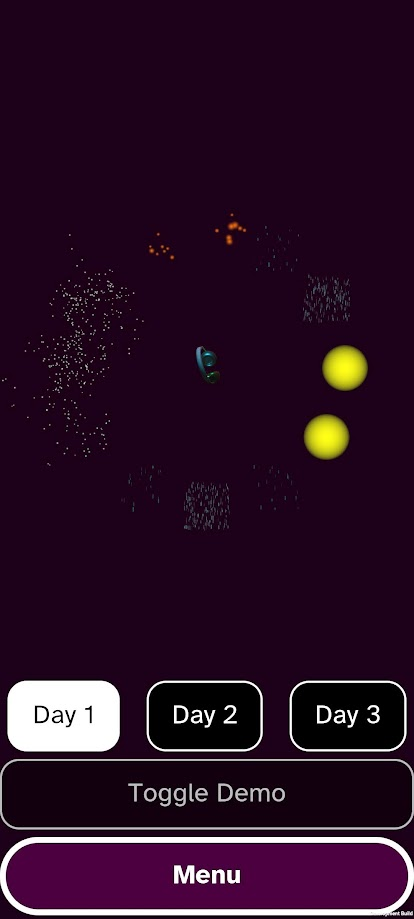
\includegraphics[width=0.3\linewidth]{images/forecast_screenshot_1.jpg}
    \caption{A screenshot of Forecast Mode in Look At The Sky}
    \label{fig:forecast_screenshot}
\end{figure}
%==================================================================================================================================
\chapter{Evaluation} 
%How good is your solution? How well did you solve the general problem, and what evidence do you have to support that?

This chapter details the rounds of evaluation conducted throughout the development phase of this project.

\section{Audio Association Survey} \label{sec:audio_survey}
\subsection{Experimental Setup}
The first evaluation conducted was an online questionnaire designed to test the set of sound effects that had been designed for the app. The aim of the survey was to investigate how effective the sounds were at communicating the weather condition they were designed to represent.

Participants were presented with eight 20-second sound clips one at a time - each without their corresponding visual effect and generically labelled (Sound A - Sound H). After hearing each clip the participant was asked which weather condition they thought was being represented as well as how intense they perceived the weather to be from the sound on a scale of 1 (Mild) to 5 (Heavy). There was also a space for participants to submit feedback or comments about each sound.

The survey was distributed digitally via Google Forms and could be completed in unsupervised conditions by participants from their own devices.

\subsection{Participants}

The survey had 13 respondents in total. No demographic data was collected from participants in this round of evaluation.

\subsection{Results}

This section presents the findings of this survey for each sound effect individually, in the order they were presented to participants in the questionnaire.

\begin{figure}
    \centering
    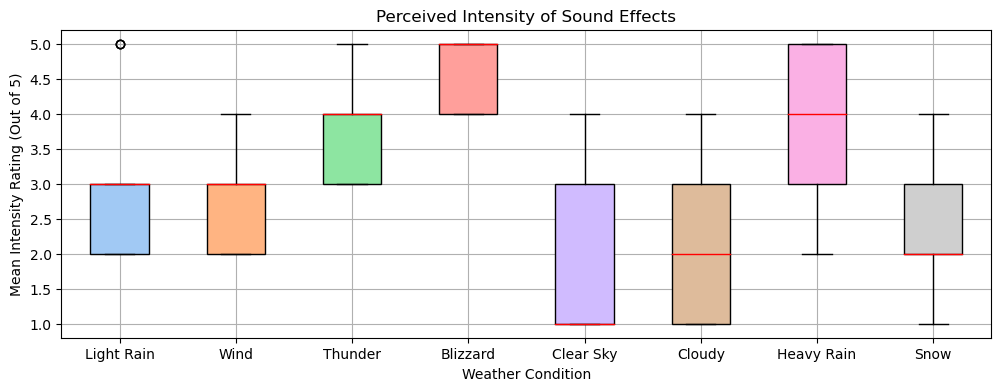
\includegraphics[width=\linewidth]{images/graphs/Intensities.png}
    \caption{Boxplot depicting the distribution of responses to the 'intensity' question for each sound effect.  1 is considered mild and 5 is considered heavy weather.}
    \label{fig:intensities_graph}
\end{figure}

\subsubsection{Sound A - Light Rain:}

All 13 Participants correctly identified this sound as representing rain. One participant (Participant 3) specifically described it as 'Heavy Rain' while another said 'A rainy morning, light rain' which most closely describes the intended effect of the sound.

3 of the 13 Participants gave this sound an intensity rating of 5 (Heavy), including the participant who initially described the sound as 'Heavy Rain'. This could have been caused by the lighter rain effect appearing before the heavy rain in the survey and thus the participants did not yet have anything to compare it to, randomising the order in which sounds were presented to the participant may have mitigated this issue.

\subsubsection{Sound B - Wind:}

All 13 participants also correctly identified Sound B as representing wind.

\subsubsection{Sound C - Thunder:}

All participants successfully identified this sound as representing a thunderstorm.

\subsubsection{Sound D - Blizzard:}

Only 3 of the 13 participants identified this effect as blizzard. The majority (9) associated this sound with intense, gale force winds. 

This indicated that I needed to reduce the volume of the wind clip in this effect and increase the volume of the 'snowier' sounds (footsteps crunching through snow and bell sounds).

\subsubsection{Sound E - Sun:}
11 of the 13 participants identified this effect as representing a clear or sunny day. At the point this evaluation was conducted the day and night cycle on the clear sky effect had not yet been implemented, so participants in this evaluation only heard what would become the 'daytime' variant of the effect.

A few participants at this stage (Participants 3, 5, 9 and 12) noted that the sound of a breeze that is present in this effect could suggest that the weather condition being communicated here is a light wind instead of a generally clear day. In later iterations of the sound the volume of this breeze is heavily reduced and more bird songs are layered on  top of this clip.

\subsubsection{Sound F - Cloudy:}
Sound F was predicted to be the least identifiable sound of the group since it was the most difficult to design and has the fewest natural association with sound. This turned out to be accurate as only 1 participant correctly identified this sound as representing cloudy weather.

The results of this survey prompted substantial reworking of the cloud effect make it more recognisable to users.

\subsubsection{Sound G - Heavy Rain:}

Similarly to the lighter rain example all participants were able to identify this clip as rain. 

Figure \ref{fig:intensities_graph} shows that in general participants could tell that this was a heavier rainfall than the lighter rain, with a higher mean of \num{3.923077} as opposed to \num{3.000000}.
The responses for sound G were noticeably more varied, with an interquartile range of \num{2.0} than for sound A with an interquartile range of \num{1.0}.

\subsubsection{Sound H - Light Snow: }

12 of the 13 participants correctly identified this sound as representing snow.

\subsection{Issues}
The question which asked the participant which weather condition they associated with each sound was made a free-text question to discourage picking an option at random if the participant was unsure. This made the analysis of the findings more difficult as similar responses were split up in Google Forms' automatically generated results page (i.e. 'Snow', 'snow' and 'snowy' were treated as different answers).

\section{Main Evaluation} \label{sec:main_eval}

\subsection{Experimental Setup}
The aim of this evaluation was to investigate the usability and functionality of the application.
This experiment was split into two parts - a think-aloud evaluation and an online survey. Participants were asked to fill in the demographic information section of the survey before they used the app.

I adopted a within-subjects design for this experiment due to a relatively small pool of participants. All participants experienced the app using both the NC700 Headphones and Bose Frames. The order in which participants used the two devices was alternated to reduce confounding of the results due to sequence effects.
In the think-aloud portion of the experiment participants used the app with both headsets and were guided to complete a small set of tasks while vocalising their thought processes as much as possible.

While using the app with each headset, participants were asked to: \begin{itemize}
    \item Use the \textit{look up} gesture to hear the current weather on each of the three example days.
    \item Use the \textit{look up} gesture to hear a variety of weather effects in \textbf{demo mode}.
    \item Take a short walk around the room while listening to weather effects either from the example days or from demo mode.
    \item Adjust gesture sensitivity and delay settings to a comfortable level using the settings menu if required.
    \item Enable and use forecast mode using the default setting of 8 hours.
    \item Change the forecast mode setting to find the most comfortable option.
\end{itemize}

After completing the tasks, I allowed participants to freely use the app for as long as they wished before continuing with the experiment.

The remainder of the survey asked the participants questions pertaining specifically to their experience using the app during the think aloud section of the evaluation.

Quantitative data was collected using both Likert scale questions and multiple choice questions while qualitative data was collected using a combination of free-text questions in the survey and unstructured interview-style questions from the evaluator.

Some of the Likert scales were inverted to discourage participants from simply clicking through questions without properly reading them. In these cases the most positive rating would be 1 and the least positive would be 5. In processing, these responses were flipped so 5 was the most positive response for all questions.

\subsection{Participants}
11 participants were used for this study, all falling within the age range of 18-24. 

9 participants considered themselves "tech savvy" people. This was to be expected as most of the participants were fellow Computer Science students.

Most participants had no previous experience with Augmented Reality equipment and fewer still (only Participant 4) had any experience with audio only AR - citing the spatial audio capabilities of some recent Apple devices, which they used regularly. However, the uses of that system are quite different from those being presented in this evaluation and this prior experience did not appear to have an impact on their responses to the survey.

\subsection{Results \& Discussion}
\subsubsection{Overall: }The majority of participants (8 of the total 11) preferred using the Bose Frames to the NC700 Headphones. There was a variety of reasons for this preference including the fit of the device (the Bose NC700s lack a lot of adjustability in the headband and so some participants mentioned needing to hold them while looking up) and the quality of the head tracking, which is discussed in section \ref{sec:gesture_detection_eval}.

The forecast mode functionality was also favourably received by participants across both headsets, scoring an average rating of \num{4.0} with a relatively small standard deviation value of \num{0.774596669
} when asked how useful they believed the feature would be in practice. However some users did struggle to pick out where individual sounds were coming from especially in its default setting which played 8 sounds from 8 points and preferred the mode which only plays 4 sounds. Some sounds were found to overpower others in forecast mode - especially blizzard - and were reduced in volume for the final iteration.

\subsubsection{Gesture Detection: }\label{sec:gesture_detection_eval}

\begin{figure}[htb!] 
    \centering
    \begin{subfigure}[b]{0.6\textwidth}
        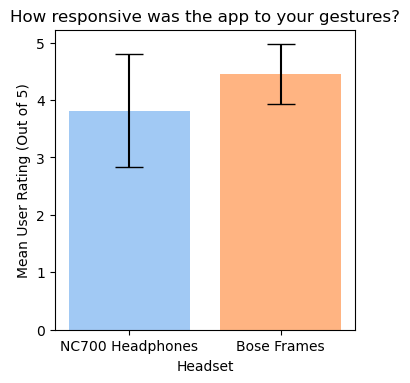
\includegraphics[width=\textwidth]{images/graphs/gesture_response_graph_small.png}
        \caption{Bar plot showing the mean responses to the Likert scale question "How responsive was the app to your gestures?" for each headset.}
        \label{fig:syn1}
    \end{subfigure}
    \begin{subfigure}[b]{0.6\textwidth}
        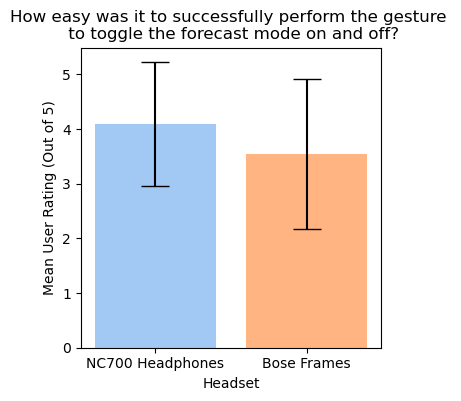
\includegraphics[width=\textwidth]{images/graphs/forecast_gesture_graph_small.png}
        \caption{Bar plot showing the mean responses to the Likert scale question "How easy was it to successfully perform the gesture to toggle the forecast mode on and off?" for each headset.}
        \label{fig:syn2}
    \end{subfigure}
    \caption{Charts showing data collected from participants about gesture detection and response in the app. Subfigure \subref{fig:syn1} refers to overall gesture detection in the app while \subref{fig:syn2} refers specifically to the input gesture used to toggle the forecast mode. Error bars show standard deviation for each set.
    }\label{fig:gesture_dection_graphs}
\end{figure}

Figure \ref{fig:gesture_dection_graphs} shows how the gesture detection in the app responded during user testing. Overall participants found that the Bose Frames were more responsive to gestures than the NC700 headphones. This makes sense as the head tracking on the headphones was a lot more temperamental and would stop responding or need reset more often than when using the Bose Frames. This would be frustrating to the user especially in a public setting to need to constantly reset the headset.

Conversely, participants found that the headphones were actually more responsive to the input gesture than the frames due to using the touch-sensitive panel rather than the accelerometer. Many participants needed multiple tries to successfully trigger the gesture due to it needing to be tapped with significantly more force than expected. Some participants did not encounter this issue, causing noticeable variation in the responses to this question in the survey.

This experiment revealed that calculation of the gesture trigger point required further development. When using a fixed rotation value for all devices there was a noticeable difference in users' perception of that point when switching between devices. While 8 participants (\num{72.7}\%) found that the look up gesture triggered at a comfortable height when using the Frames, only 1 participant also found that the gesture activated at a comfortable height when using the headphones.

This prompted me to add functionality for dynamically adjusting the default, minimum and maximum rotation values for triggering the look up gesture based on the connected headset. The impact of this update was examined in a later experiment, detailed in Section \ref{sec:final_eval}.

\subsubsection{Audio: }

Two main facets of the audio design were examined in this experiment - the quality of the sounds themselves and the quality of the audio spatialisation.

Figure \ref{fig:audio_tracking_graph} displays how easily users were able to pick out which direction elements of the soundscape were coming from. Both the headphones and Frames achieved similar average ratings from participants (\num{2.90909} and \num{3.27273} respectively) but there was a wide spread of ratings for both headsets, suggesting that this metric is very subjective and would likely benefit from some customisation options so the user can adjust the directionality of the sound to their liking.

\begin{figure}[h!]
    \centering
    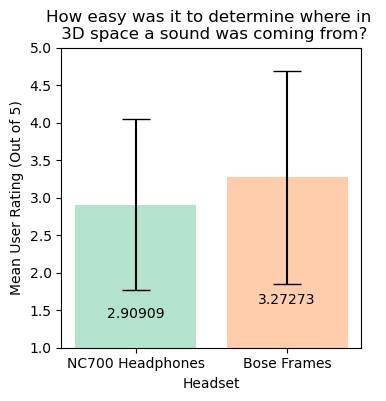
\includegraphics{images/graphs/audio_detection_small.png}
    \caption{Plot showing the average user response to the question "How easy was it to determine where in 3D space a sound was coming from?" for each of the two headsets. Error bars show the standard deviation for each set}
    \label{fig:audio_tracking_graph}
\end{figure}

Figure \ref{fig:audio_preference_graphs} Shows which weather effects participants deemed most effective at communicating its intended weather effect and which were voted least effective.
38.5\% of the total votes for most effective sound were given to the rain effects. This was to be expected as the initial evaluation showed that this effect very clearly represented rain to all participants. In this instance, it is unspecified whether both the heavy rain and lighter rain effects were equally effective.
Interestingly, the clear sky effect has a large distribution of votes for both most effective and least effective, suggesting that the calm bird noises have a much stronger association for some participants than others and should be reworked to be clearer to all users.

It is unclear what \emph{"mild"} refers to in these results, though it is likely talking about the quieter effects like cloudy or clear sky.

The Blizzard effect received 2 votes as the least intuitive sound as it was again confused for wind, suggesting that the volume wind clip in this effect should be reduced further or even removed entirely.

\begin{figure}[htb!] 
    \centering
    \begin{subfigure}[b]{0.7\textwidth}
        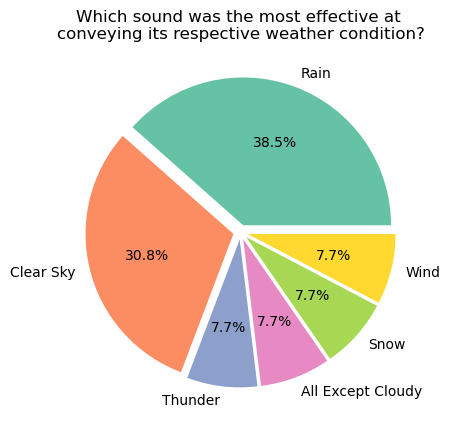
\includegraphics[width=\textwidth]{images/graphs/most_effective_pie.png}
        \caption{Distribution of participant votes for the sound that most effectively communicated its intended effect}
        \label{fig:syn1}
    \end{subfigure}
    \\
    \begin{subfigure}[b]{0.7\textwidth}
        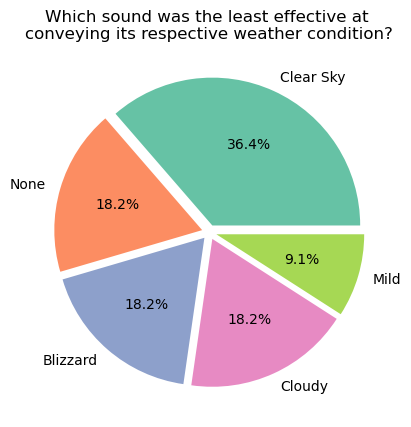
\includegraphics[width=\textwidth]{images/graphs/least_effective_pie.png}
        \caption{Distribution of participant votes for the sound that least effectively communicated its intended effect}
        \label{fig:syn2}
    \end{subfigure}
    \caption{Visualisation of participant-voted most effective and least effective sound effects. These results refer to both headset devices, as the weather effects are the same for both. Note that votes that could not be cleanly mapped to single options were included separately.
    }\label{fig:audio_preference_graphs}
\end{figure}

\subsubsection{Portability \& Social Acceptability: }
Participants were also asked about the social acceptability of the app and its interaction methods for each headset. It is important that, as a mobile application that utilises gesture control, the user can feel confident using it in a public space.

The questionnaire asked participants two Likert scale questions relating to portability and social acceptability in the headset-specific sections. Participants were asked to rate how they felt while walking around and using the app, as well as how confident they would feel using the app in a public setting.

\begin{figure}[htb!]
    \centering
    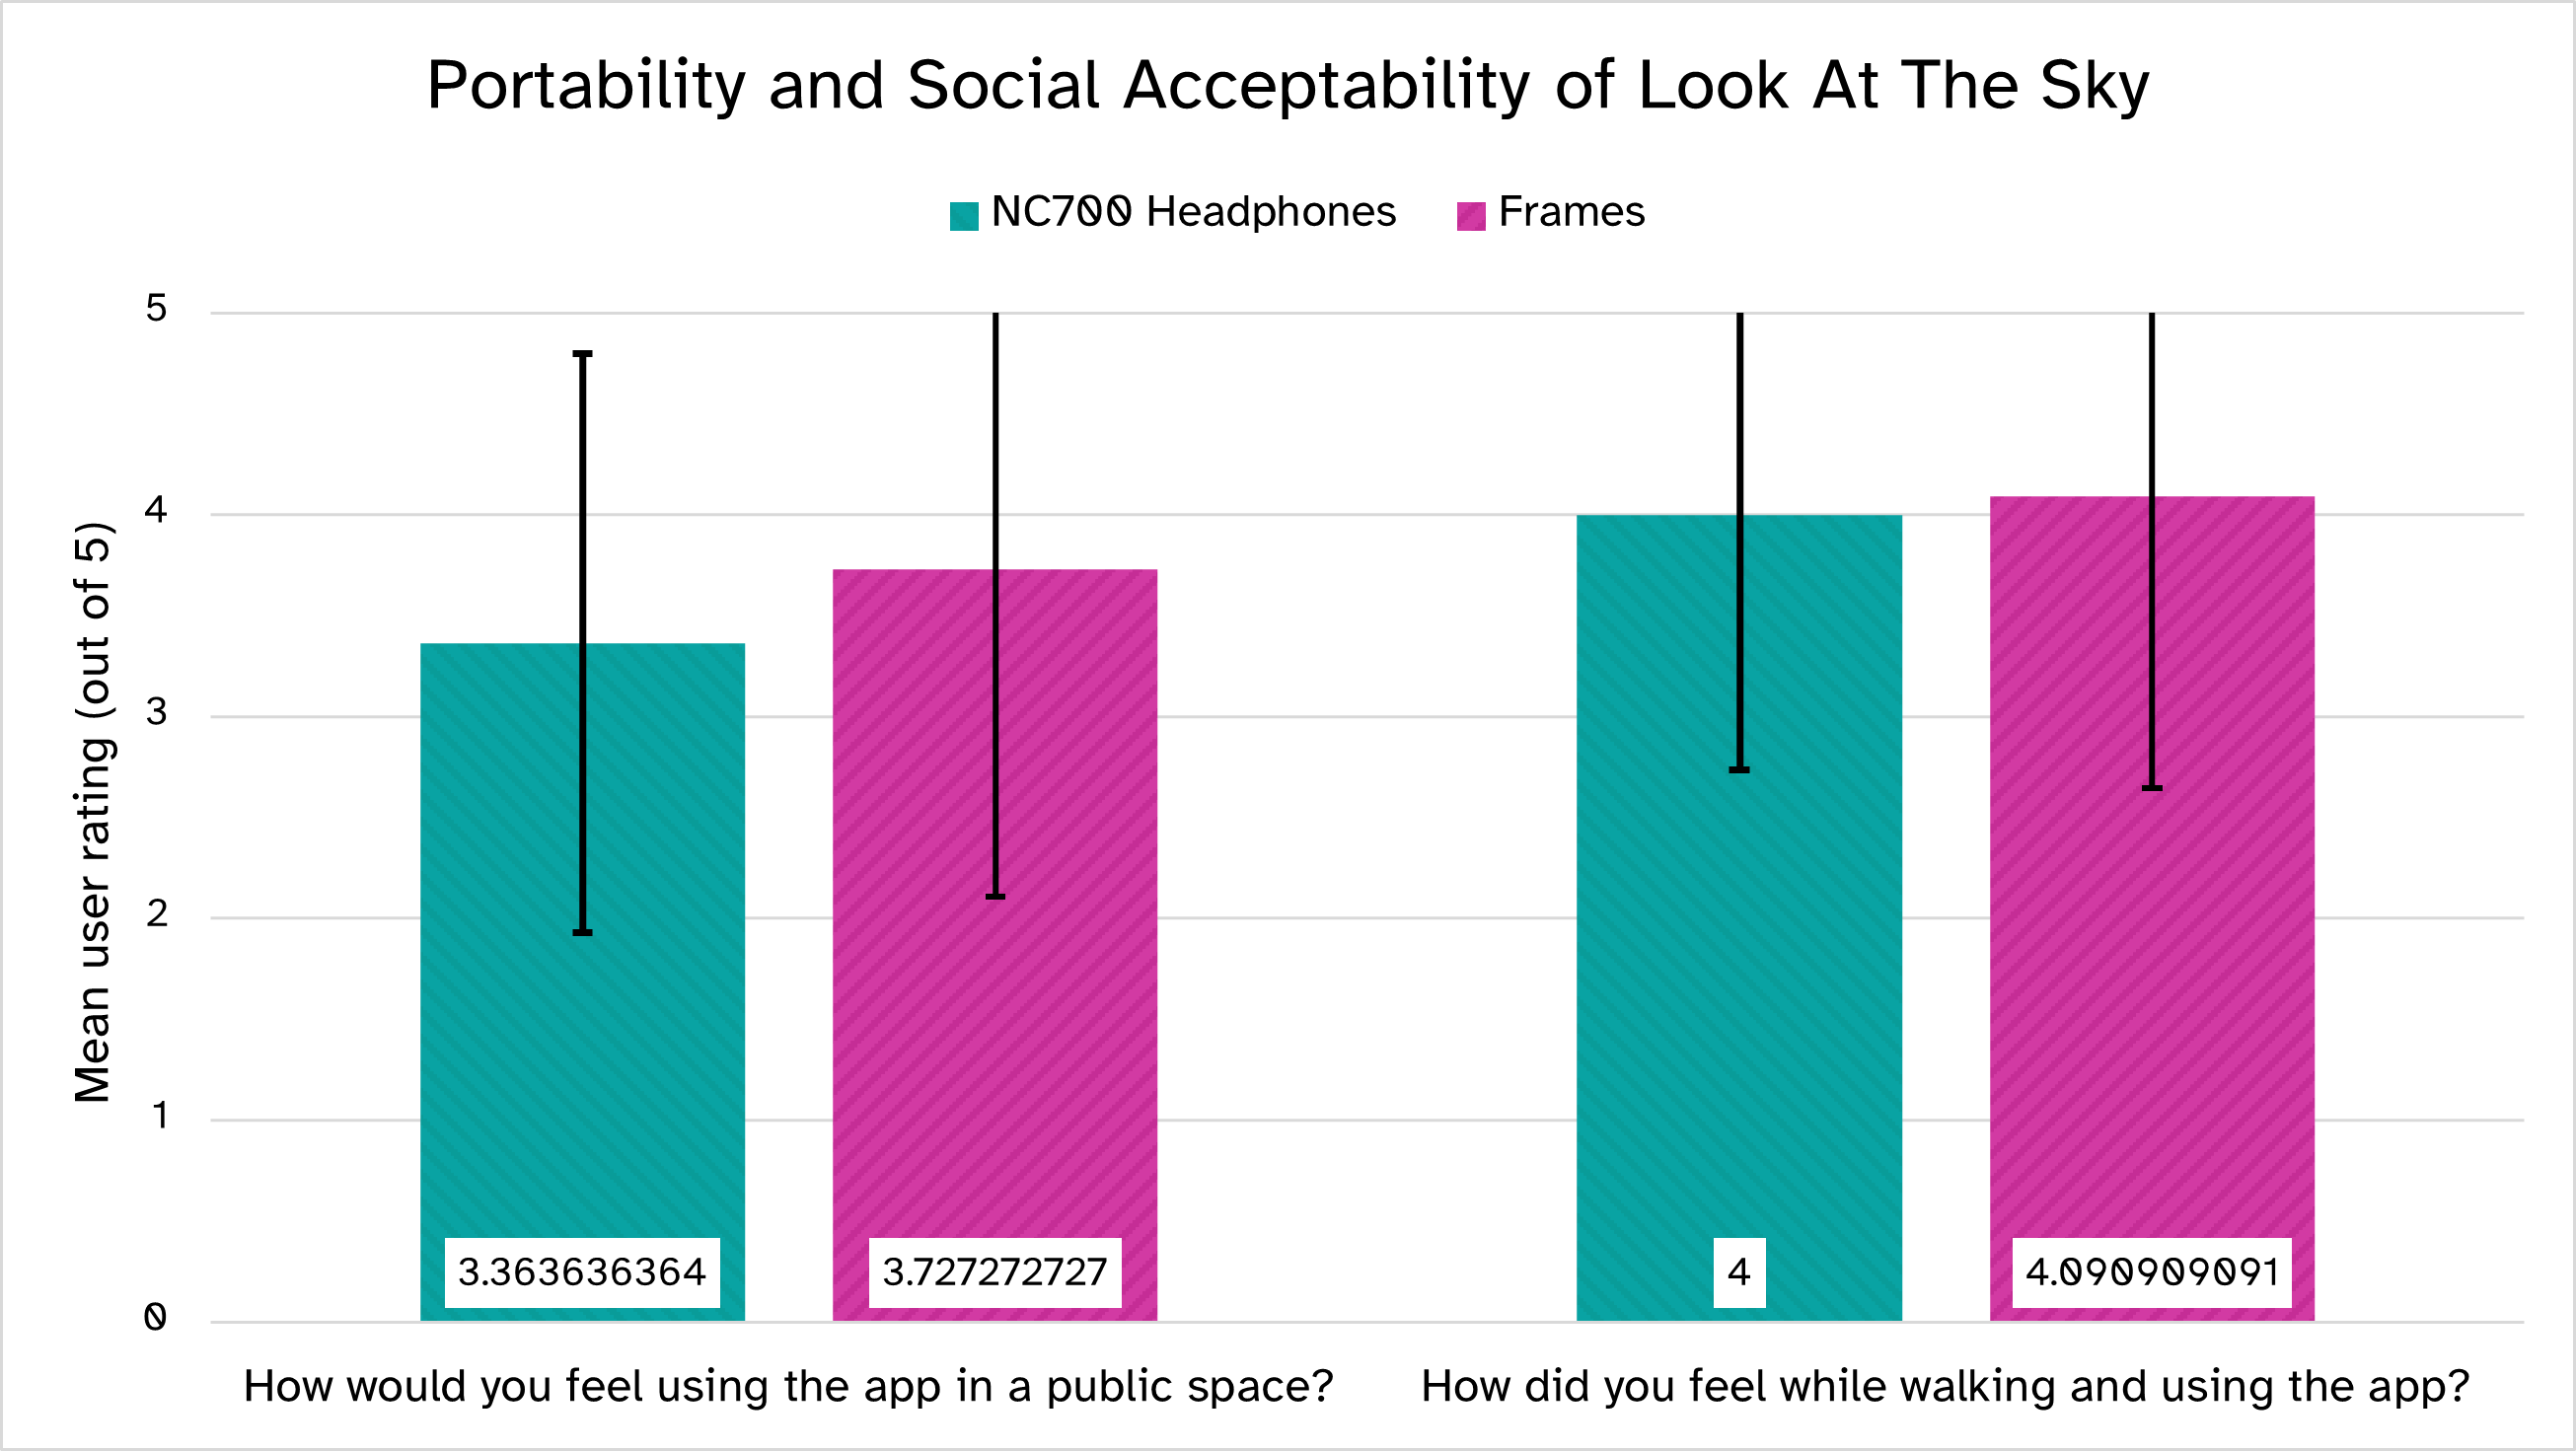
\includegraphics[width=0.9\textwidth]{images/graphs/Social acceptability graph.png}
    \caption{Mean results per headset for Likert scale questions relating to the portability and social acceptability of Look At The Sky. Error bars show the standard deviation of each set of results.}
    \label{fig:social_acceptability}
\end{figure}

As shown in Figure \ref{fig:social_acceptability}, both devices scored relatively well across the board in this portion of the experiment.

The Frames were overall preferred by users when walking around since the main gesture was significantly easier to activate and most users did not encounter issues with the fit of the glasses - whereas some participants described needing to physically hold the headphones onto their heads to stop them from falling off. This issue is exacerbated when the participant has to move around.

When walking around, several users found that the headphones were somewhat difficult to use comfortably due to the trigger point being too high. Some participants expressed concern that the extra height needed to trigger a weather effect made it difficult to see where they were going and could cause them to bump into obstacles if used in a non-controlled environment like outdoors.

As the evaluation was held indoors for participant safety, no data was actually gathered on outdoor or public use of the app and instead relied on the participant's own perception of how confident they were likely to feel in a public space.

Both headsets were, on average, rated similarly for public confidence and acceptability. The headphones gained an average rating of \num{3.363636364
} for social acceptability while the frames scored slightly higher with a mean rating of \num{3.727272727}. The spread of ratings for the frames was marginally higher, with a standard deviation of \num{1.61807967} as opposed to \num{1.433368569}.
This was a somewhat surprising result as it was expected that participants would feel significantly more comfortable in a standard pair of headphones as opposed to the more unusual Bose Frames. The reason for this confidence is likely due to the Bose Frames looking nearly indistinguishable from a normal pair of glasses at a distance.
 
\subsubsection{Quality Control \& Bugs:}This round of evaluation exposed some remaining bugs in the app that hadn't been previously identified while testing. If an effect was enabled when toggling out of demo mode, there was a chance that the effect would become stuck on. Similarly, when toggling into demo mode, the first selected sound would not properly trigger if it was the same sound that had been previously enabled.

Both of these bugs were solved by adding an extra call to \texttt{EffectController.ExitZone()} and \texttt{EffectController.DisableAll()} when switching between modes to ensure sounds do not get stuck on and also do not wrongly think they are still enabled when they aren't. This fix was also applied when switching between data sets to prevent similar issues occurring.

\subsubsection{General User Feedback \& Suggestions} \label{sec:feedback}
Participants were asked for feedback on their experience both throughout the think-aloud evaluation and towards the end of the questionnaire.

Two participants suggested an alternative gesture to trigger the current weather effect as they fought with the poorly set trigger point and poor fit of the headphones. They suggested instead turning their head to the side instead of looking straight up. This alternative gesture was never formally evaluated, though giving the user the option to choose between different trigger gestures could better accommodate those who find the default gesture uncomfortable.

Participants gave a wide variety of responses when asked what other weather effects should be included in future versions. Hail and sleet received the most votes with 3 and 2 mentions respectively. Sandstorms and a stronger wind effect were also suggested. 2 Participants wrote that all necessary weather conditions were already included, while another 2 left the question blank.

Verbal feedback given throughout the experiment was overall positive, although users did become understandably frustrated when the head tracking failed and the headset needed to be reset.

\section{Final Evaluation - Gesture Trigger Height} \label{sec:final_eval}
As the main evaluation revealed issues with the activation point of the look up gesture on the headphones, I decided to carry out a final, smaller evaluation to check that the implemented solution to this had mitigated the issue.

\subsection{Experimental Setup}
After completing a short introductory section of this evaluation's questionnaire, users were asked to use the app with each headset and complete some basic tasks.

For each headset, participants were asked to: \begin{itemize}
    \item Perform the \emph{look up} gesture at the default sensitivity and delay values.
    \item Adjust the sensitivity and delay settings to a find a comfortable height, if required.
\end{itemize}
This experiment also adopts a within-subjects design as all participants used and answered questions on both headsets. The order in which participants used each headset was again swapped for each participant to reduce sequence effects in the results.

Afterwards, participants were presented with a short questionnaire whether the gesture was triggered at too high an angle, too low an angle or a comfortable angle for their neck.

\subsection{Participants}

Only 3 Participants were used for this final evaluation, all again falling within the age range of 18-24. No other demographic information was collected from participants at this stage.

\subsection{Results \& Discussion}

All three participants found that, when using the Bose Frames with their default settings, the gesture triggered at a comfortable neck angle. This was to be expected as the default trigger value was kept the same as the main evaluation for this version. 

When using the headphones, 2 of the 3 participants found that the new default activation height was comfortable for them while Participant 1 found that the angle was still "very slightly" too high. However they also found it very easy to use the settings menu to customise the sensitivity of the gesture to their liking, giving it a rating of 5.

While this suggests that the initial values could benefit from further research and refinement, the results of this final evaluation are promising.




%==================================================================================================================================
\chapter{Conclusion}    

\section{Summary}
%Summarise what you did; answer the general questions you asked in the introduction. What did you achieve? Briefly describe what was built and summarise the evaluation results.
This project focused on exploring and demonstrating a possible application of audio augmented reality in an everyday context. The final product - Look At The Sky - added spatial audio functionality to the commonly performed act of checking the weather as well as gesture control to free up the user's visual attention during use.

By looking up the user could hear a spatial audio effect representing the current weather, or by performing an input gesture on their headset, they could experience simplified versions of the current and forecast weather effects positioned in 360$^\circ$ around their head. 

Evaluation demonstrated that Look At The Sky was mostly successful in creating effective, immersive 3D soundscapes to communicate the weather, however some sounds were harder than others for users to correctly intuit their meanings. Weather conditions that naturally lack sound associations - typically milder weathers like clouds or sun - are much harder to communicate through an auditory interface and would limit the practical applications of this software.

The custom gesture detection script worked well when the gyroscope on the headset was properly calibrated. Users were easily able to find a comfortable point for them to trigger the gesture and appreciated the level of gesture customisation offered by the app.

\section{Reflection}
%Discuss what went well and what didn't and how you would do things differently if you did this project again.
The sound design - though obviously not perfect - is something I think has been successful in this process. Some weather effects like rain, wind and thunder were well received by users who participated in evaluations and are generally pleasant soundscapes to listen to when trying to relax or unwind.

Evaluation went smoothly overall, although there were some questions in the main evaluation that were asked for one headset and not the other - making them unusable in analysis - due to an error made when creating the questionnaire. Ideally the experiments should have used more participants from different age groups and backgrounds with augmented reality to obtain more generalisable results about the usability of the app with different demographics.

The main hindrance faced during this project was the Bose AR hardware and SDK. Look At The Sky was tested primarily on the 1st Generation Frames \emph{"Rondo"} which were released in 2019. The app faced multiple issues with sensor data and gyroscope connection which may have been fixed in later hardware revisions, therefore it may have been beneficial to test using the later hardware generation.

During the project I spent a considerable amount of time fixing my personal laptop because I didn't realise how easy it would be to acquire a loaned laptop from the school. If I had asked for one sooner I wouldn't have spent quite so many days unable to work on my project due to needing to fix my personal machine.

\section{Future work}
%Discuss what you would do if you could take this further -- where would the interesting directions to go next be? (e.g. you got another year to work on it, or you started a company to work on this, or you pursued a PhD on this topic)
With more time, this design concept could be refined and iterated upon to create a product more suited for deployment.

The app should be updated to call a web API for the current weather in the user's location instead of a set of hard-coded JSON data sets, although these were more useful for running controlled user tests during this project.

As discussed in section \ref{sec:feedback}, there are several weather conditions absent from the final iteration of the project such as hail and sleet. If Look At The Sky was to be compatible with external weather data then it would need to support a much wider range of weather conditions than the 8 demonstrated in this project. In addition, more effects would need to have different variations to show different intensities of weather. For example a light breeze versus gale force winds.

There were some further goals defined in the functional requirements that were ultimately not implemented during this project, but would be useful inclusions. Providing the user with a subtle, customisable audio notification if rain, thunder or some other weather condition was forecast to begin shortly would be a good way to add extra utility to the app when the user is not actively performing gestures without demanding too much of their attention.

In the future this app would need to abandon the Bose AR ecosystem, since it is no longer supported, and would overall benefit from becoming more platform-agnostic if it were to become truly useful as an everyday app.
%==================================================================================================================================
%
% 
%==================================================================================================================================
%  APPENDICES  

\begin{appendices}

\chapter{Audio Source Attribution} \label{adx:audiosources}

Rain \begin{itemize}
    \item Individual raindrops - \url{https://soundbible.com/1126-Water-Drop.html} - Attribution 3 (Edited to different pitches)
    \item Light background rain - \url{https://freesound.org/s/607070/} - Creative Commons 0
    \item Drum (for individual raindrops) - \url{https://freesound.org/people/karolist/sounds/371192/} - CC0
    \item Heavier rain - \url{https://freesound.org/s/531947/} - Attribution 4
\end{itemize}


Thunder \begin{itemize}
    \item Thunder 1 - \url{https://sound-effects.bbcrewind.co.uk/search?q=NHU9752541} - BBC RemArc License (Non-commerical) (Cut down)
    \item Thunder 2 - \url{https://sound-effects.bbcrewind.co.uk/search?q=NHU05009110} - BBC RemArc License
    \item Thunder 3 - \url{https://freesound.org/people/straget/sounds/527664/} - Attribution 4
\end{itemize}


Snow \begin{itemize}
    \item Bells - \url{https://freesound.org/s/538787/} - Attribution 4
    \item Footsteps in Snow - \url{https://sound-effects.bbcrewind.co.uk/search?q=07004055} - BBC RemArc License
    \item Hand Bell - \url{https://freesound.org/people/InspectorJ/sounds/339814/}- Attribution 4
    \item Blizzard - \url{https://sound-effects.bbcrewind.co.uk/search?q=07061030} - BBC RemArc License
    \item Yet more footsteps - \url{https://sound-effects.bbcrewind.co.uk/search?q=07004064} - BBC RemArc License
\end{itemize}


Sun \begin{itemize}
    \item Summer Ambience (Birds etc) - \url{https://sound-effects.bbcrewind.co.uk/search?q=07030059} - BBC RemArc License
    \item Seagull for beach vibes - \url{https://sound-effects.bbcrewind.co.uk/search?q=NHU05010042} - BBC RemArc License
\end{itemize}


Wind \begin{itemize}
    \item Wind ambience - \url{https://sound-effects.bbcrewind.co.uk/search?q=NHU9322987} - BBC RemArc License (Cut down)
    \item Heavy Wind - \url{https://sound-effects.bbcrewind.co.uk/search?q=NHU05039063} - BBC RemArc License
    \item Medium Wind - \url{https://freesound.org/people/kangaroovindaloo/sounds/205966/} - Attribution 4
    \item Windchimes - \url{https://freesound.org/s/398495/} - CC0
\end{itemize}


Cloudy \begin{itemize}
    \item Dreamy ambience - \url{https://freesound.org/people/EgilSG/sounds/517302/} - Noncommercial 4
    \item Breeze and geese - \url{https://freesound.org/s/217429/} - Noncommercial 3
    \item More wind - \url{https://freesound.org/s/181253/} - CC0
    \item Autumn vibe - \url{https://freesound.org/people/Fedor_Ogon/sounds/649230/} - CC0
    \item Lighter Breeze - \url{https://freesound.org/people/johanwestling/sounds/460178/} - CC0
    \item European Birds - \url{https://freesound.org/people/ValentinPetiteau/sounds/563547/} - CC0
\end{itemize}


Clear Night \begin{itemize}
    \item Crickets and owl 1 - \url{https://freesound.org/people/opalmirage/sounds/666760/} - CC0
    \item Tawny Owls - \url{https://freesound.org/people/Eelke/sounds/593654/} - Noncommerical 4.0
    \item Classic Owl - \url{https://freesound.org/people/Breviceps/sounds/465697/} - CC0
\end{itemize}

Supplementary Earcons - ALL PROVIDED BY BOSE SDK \begin{itemize}
    \item Look Up Gesture Triggered - "button\_interact"
    \item Forecast View Enabled - "spawn"
    \item Forecast View Disabled - "collect"
\end{itemize}




\chapter{Ethics Checklist}
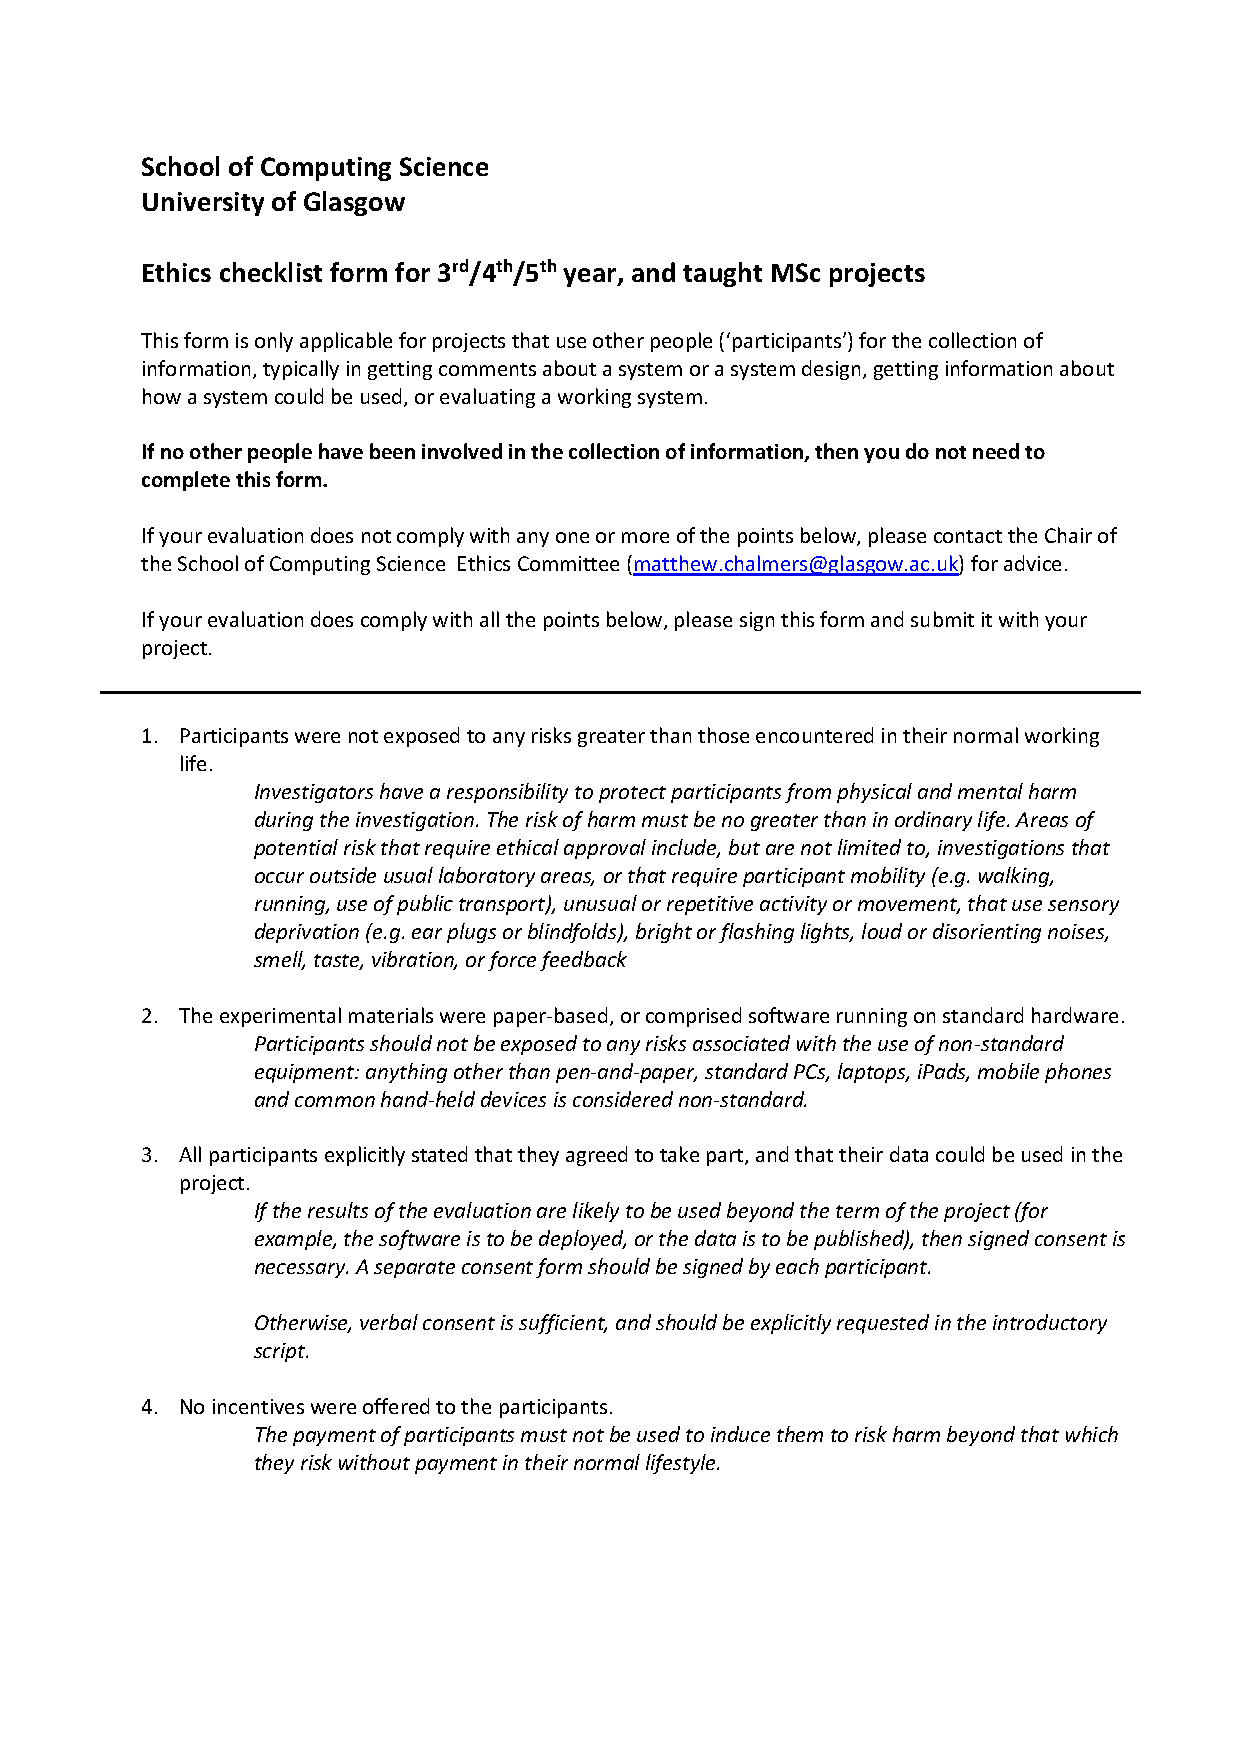
\includepdf[pages={-}]{images/pdfs/ethics_form_signed.pdf}

\chapter{Evaluation Consent Form}
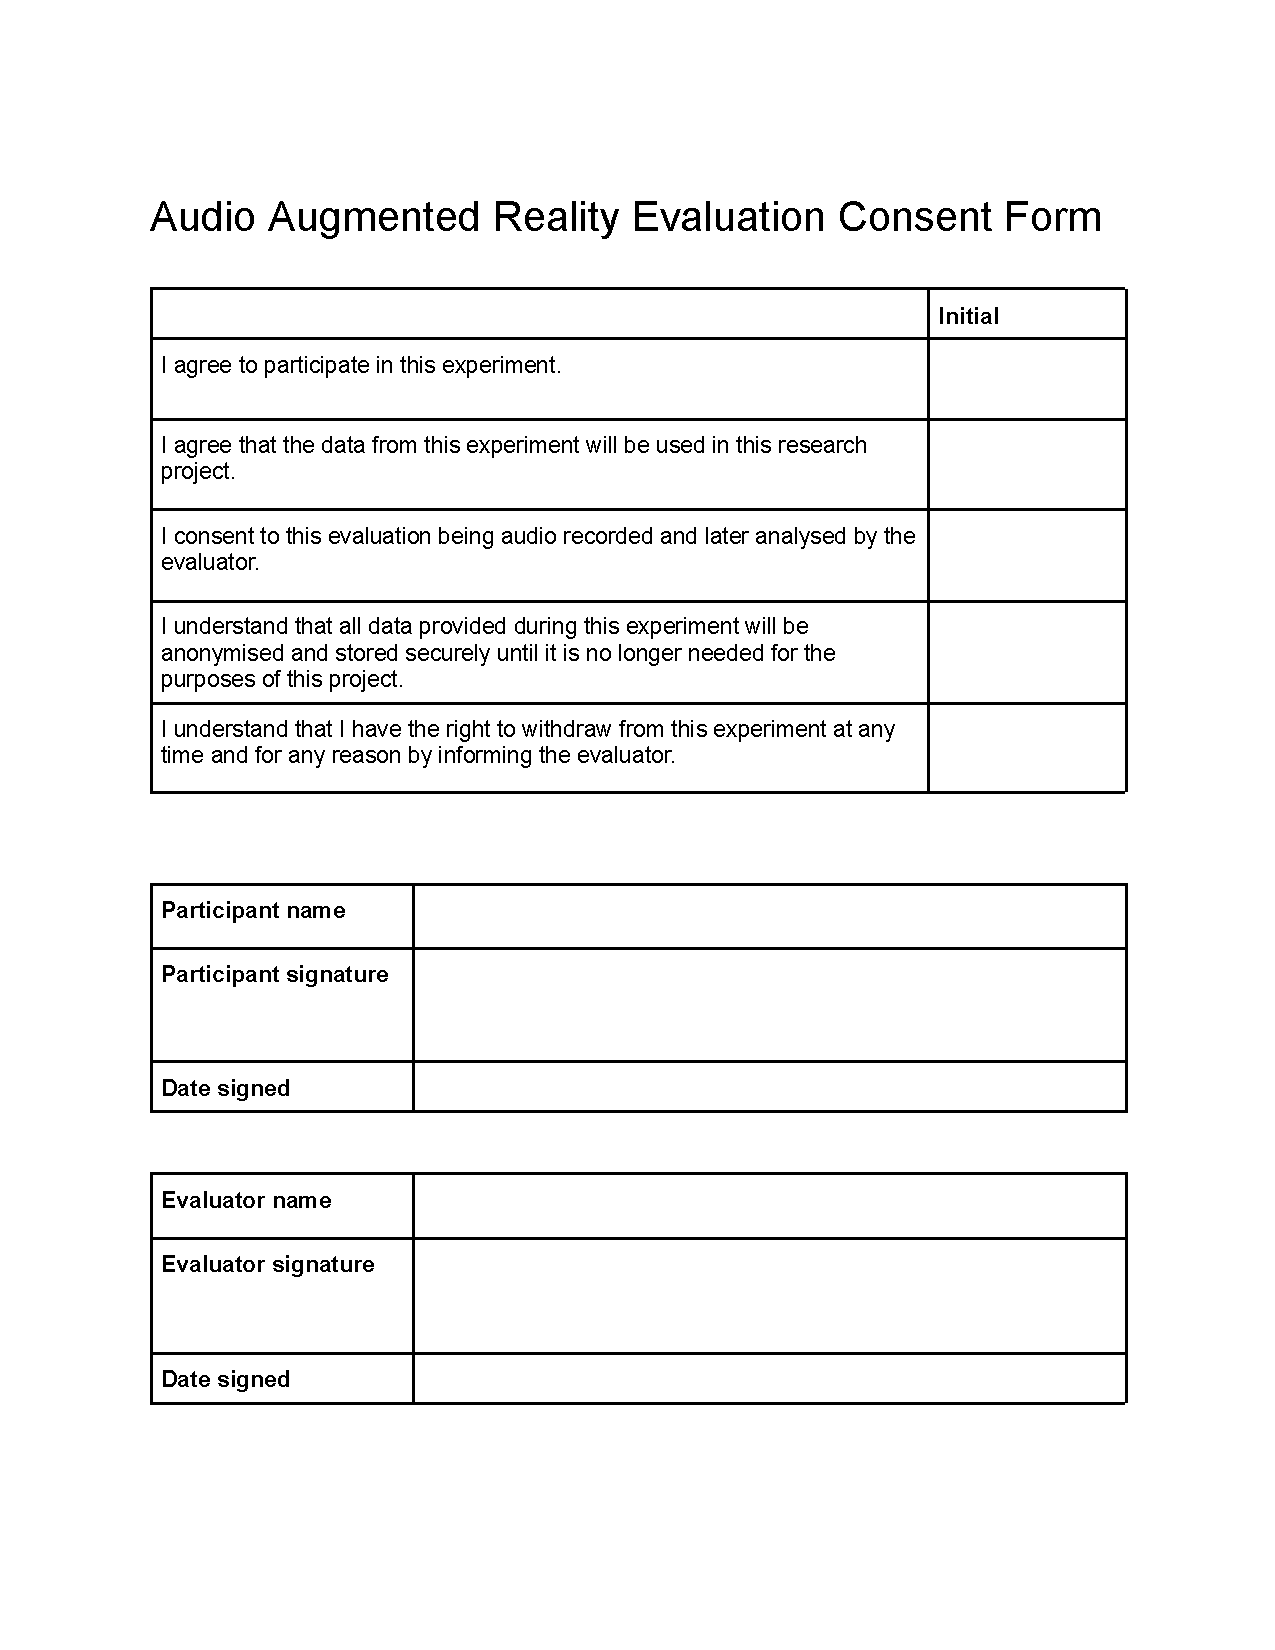
\includepdf[pages={-}]{images/pdfs/blank consent form.pdf}

\chapter{Build Instructions \& File Structure}

\section{File Structure}
The majority of the source files are a mix of proprietary Unity file types and C\# script files.

The code can be found in \texttt{Weather App} - The rest is mostly library files and project configuration data.
\begin{itemize}
    \item \texttt{Assets} contains the bulk of the project code and materials.
    \item \texttt{Audio} contains the sound files used in the app (except those included with the Bose SDK).
    \item \texttt{Bose} contains the Bose SDK and its associated files.
    \item \texttt{Fonts} contains the font files and Unity Font Assets needed to render text on screen.
    \item \texttt{Prefabs} contains the Unity prefab files for the simplified weather sounds used in Forecast Mode.
    \item \texttt{Resources}` contains the JSON files storing three example days of weather.
    \item \texttt{Scenes} contains the Unity scene.
    \item \texttt{Scripts} contains all of the C\# code written for this project.
    \item \texttt{TextMeshPro} contain package configuration data for TextMeshPro.
    \item \texttt{UI} contains UXML and USS files used to build menus and buttons.
    \item \texttt{UI Toolkit} contains configuration data for UI Toolkit.
\end{itemize}

\section{Build Instructions}

\subsection{Requirements}
\begin{itemize}
    \item Requires Bose Frames (with cable if running on PC) or Bose NC700 Headphones.
    \item Unity version \texttt{2021.3.11f1} with \texttt{Android Build Support} module installed.
    \item Android Phone (Tested on OnePlus 8T running Android 12 (API 31)) with developer options and USB debugging enabled.
    \item Build tested from Windows 10 and 11.
\end{itemize}

\subsection{Build Steps}

To build to Android device from Unity: \begin{itemize}
    \item Plug in Android phone, ensure media transfer and USB debugging are on (on the phone).
    \item Ensure Android is selected in Build Settings in Unity.
    \item Select `Build and Run`.
    \item Save the APK if prompted.
    \item Wait To Complete
    \item Once built and installed, it can be launched from the app drawer like any app.
\end{itemize}


 The build error `Destroy() may not be called from edit mode! Use DestroyImmediate() instead.` occasionally appears and is caused by a known bug in the editor. It can be fixed by building again.

\subsection{Test Steps}

Running on Android Device: \begin{itemize}
    \item Connect Bose AR enabled headset via Bluetooth to the phone before opening the app - NOTE: Try to look straight forward when powering on the headset to set the gyroscope properly.
    \item The app will ask for location permission on first startup - \textbf{NOTE: This is ONLY for the BLE connection between the headset and the mobile device and the app doesn't read or process any location data at all (hence when running through Unity only it doesn't need this since Bluetooth isn't involved).}
    \item Connect the headset via BLE using the GUI.
    \item After the headset has connected the on-screen model should copy its movements.
\end{itemize}

Running on PC via Unity: \begin{itemize}
    \item Open the project folder (Weather App) in Unity via Unity Hub.
    \item Connect the Bose Frames to the PC via the included USB-Magnet cable.
    \item Click the Play button at the top of the Unity window. Try to hold the glasses level as they power on and connect.
    \item The glasses will connect and the on-screen model should match its movements
\end{itemize}

Note that only the Bose Frames are able to connect to Unity over USB.

Instructions for using the app can be found in \texttt{manual.md}.

\section{Usage Instructions}

\subsection{How To Use}
On startup, the connected Bose device can be connected to the app via the provided GUI. There will be both an audio and graphical confirmation when the headset has successfully connected to the app.

(If wearing the headset) Look up and you should hear a confirmatory sound effect, followed by a 3D weather effect. The effect should continue for as long as you look up.

There are three example datasets which use the current time to pull a weather effect. These can be freely switched between using the \texttt{Set 1}, \texttt{Set 2} and \texttt{Set 3} buttons.

The `Demo` button toggles a demo mode where any of the available sounds can be enabled.

By \textbf{firmly} double tapping the right arm of the Frames or tapping and holding the touch panel on the right earcup of the NC700 headphones you can enter Forecast Mode. Sounds will appear in a ring around your head - in front of you is the current weather and these sounds then progress in one hour increments.

It is beneficial to try and pick out one sound, and then try to follow it as you move your head.

\subsection{Customise}
The \texttt{Menu} button opens a settings menu that allows you to customise aspects of the experience.

By turning up \texttt{Gesture Sensitivity} we lower the height at which the look up gesture triggers.

By turning up \texttt{Effect Off Delay} we increase the distance the head can travel back down before turning the effect off.

By switching between the different settings of \texttt{Forecast Mode} we can adjust how may hours of weather are included in the Forecast view.

\subsection{Troubleshooting}
It is best (when running the app from Android and using Bluetooth to connect to the headset) to power on and connect to the device before opening the app. Try to keep the headset as level as possible when powering it on.
If the sound activates when looking down instead of up, rotate the headset \textbf{360 degrees once}. This can often fix the issue.

If all else fails, close the app, power off and reconnect the headset.

\end{appendices}

%==================================================================================================================================
%   BIBLIOGRAPHY   

% The bibliography style is agsm (Harvard)
% The bibliography always appears last, after the appendices.

\bibliographystyle{agsm}

% Force the bibliography not to be numbered
\renewcommand{\thechapter}{0} 
\bibliography{l4proj}

\end{document}
